% autosam.tex
% Annotated sample file for the preparation of LaTeX files
% for the final versions of papers submitted to or accepted for 
% publication in AUTOMATICA.

% See also the Information for Authors.

% Make sure that the zip file that you send contains all the 
% files, including the files for the figures and the bib file.

% Output produced with the elsart style file does not imitate the
% AUTOMATICA style. The style file is generic for all Elsevier
% journals and the output is laid out for easy copy editing. The
% final document is produced from the source file in the
% AUTOMATICA style at Elsevier.

% You may use the style file autart.cls to obtain a two-column 
% document (see below) that more or less imitates the printed 
% Automatica style. This may helpful to improve the formatting 
% of the equations, tables and figures, and also serves to check 
% whether the paper satisfies the length requirements.

% Please note: Authors must not create their own macros.

% For further information regarding the preparation of LaTeX files 
% for Elsevier, please refer to the "Full Instructions to Authors" 
% from Elsevier's anonymous ftp server on ftp.elsevier.nl in the
% directory pub/styles, or from the internet (CTAN sites) on
% ftp.shsu.edu, ftp.dante.de and ftp.tex.ac.uk in the directory
% tex-archive/macros/latex/contrib/supported/elsevier.


%\documentclass{elsart}               % The use of LaTeX2e is preferred.

\documentclass[twocolumn]{autart}    % Enable this line and disable the 
% preceding line to obtain a two-column 
% document whose style resembles the
% printed Automatica style.

\usepackage{graphicx}          % Include this line if your 
% document contains figures,
%\usepackage[dvips]{epsfig}    % or this line, depending on which
% you prefer.
\usepackage[T1]{fontenc}
\usepackage{arydshln}
\usepackage{tikz}
\usepackage[english]{babel}
\usepackage{amsmath,amssymb,amsfonts}
\usepackage{algorithm}
\usepackage[algo2e,lined,norelsize]{algorithm2e}
\usepackage{dsfont}

\newtheorem{theorem}{Theorem}[section]
\newtheorem{lemma}{Lemma}[section]
\newtheorem{proposition}{Proposition}[section]
\newtheorem{remark}{Remark}[section]
\newtheorem{corollary}{Corollary}[section]
\newtheorem{definition}{Definition}[section]


\begin{document}
	
	\begin{frontmatter}
		%\runtitle{Insert a suggested running title}  % Running title for regular 
		% papers but only if the title  
		% is over 5 words. Running title 
		% is not shown in output.
		
		\title{Network-Realized Model Predictive Control\\ Part I: NRF-Enabled Closed-loop Decomposition\vspace{-11mm}} 
		
		% Part II: Distributed Constraint Management
		
		% Title, preferably not more 
		% than 10 words.
		
		%\thanks[footnoteinfo]{This paper was not presented at any IFAC 
			%meeting. Corresponding author M.~T.~Cicero. Tel. +XXXIX-VI-mmmxxi. 
			%Fax +XXXIX-VI-mmmxxv.}
		
		\author[L2S]{Andrei Speril\u a}\ead{andrei.sperila@centralesupelec.fr},    % Add the 
		\author[L2S]{Alessio Iovine}\ead{alessio.iovine@centralesupelec.fr},               % e-mail address 
		\author[L2S]{Sorin Olaru}\ead{sorin.olaru@centralesupelec.fr},  % (ead) as shown
		\author[L2S]{Patrick Panciatici}\ead{patrick.panciatici@ieee.org}  % (ead) as shown
		
		\address[L2S]{Laboratoire des Signaux et Syst\`emes, CentraleSup\'elec, Paris-Saclay University, Gif-sur-Yvette, France\vspace{-8mm}}  % Please supply                                              
		%\address[Rome]{Senate House, Rome}             % full addresses
		%\address[Baiae]{The White House, Baiae}        % here.
		
		
		\begin{keyword}                           % Five to ten keywords,  
			Distributed control; convex optimization; model predictive control; networked systems; scalable implementations.   \vspace{-2mm}            % chosen from the IFAC 
		\end{keyword}                             % keyword list or with the 
		% help of the Automatica 
		% keyword wizard
		
		
		\begin{abstract}
			A two-layer control architecture is proposed, which promotes scalable implementations for model predictive controllers. The bottom layer is based upon a distributed feedback-feedforward scheme, which directs the controlled network's information flow according to a pre-specified communication infrastructure. Explicit expressions of the resulting closed-loop maps are obtained and an offline model-matching procedure is proposed for the design of the first layer. The obtained control laws are deployed via distributed state-space-based implementations, and the resulting closed-loop models enable predictive control design for the constraint management procedure described in our companion paper.			
			\vspace{-5mm}
		\end{abstract}
		
	\end{frontmatter}
	
	\section{Introduction}\label{sec:intro}\vspace{-3mm}
	
	\subsection{Context and Motivation}
	\label{subsec:true_intro}\vspace{-3mm}
	
	In recent years, distributed control has received significant attention in system-theoretic literature. While a number of techniques have emerged in this field (see \cite{Luca3} for a discussion on the most prominent approaches), the problem of implementing Model Predictive Control (MPC) in a \emph{distributed} manner (in which separate subcontrollers exchange \emph{local} information) is still an actively investigated topic. Notably, the procedure formalized in \cite{DMPC1} and \cite{DMPC2}, which is based upon one of the approaches discussed in \cite{Luca3}, proposes a solution in which MPC-like policies are built using a parametrized distributed control architecture (see \cite{SLS}). With the idea of employing layered control schemes rapidly gaining traction \cite{layer_survey}, the need for a theoretical framework which takes into account the interplay between the different layers of the control algorithm becomes apparent.\vspace{-3mm}
	
	\subsection{Scope of Work}
	\label{subsec:prob_st}\vspace{-3mm}
	
	The problem being tackled in this manuscript, and in its companion paper \cite{part2}, is that of employing a class of distributed controllers (see \cite{Luca3} for a general overview) based upon the celebrated \emph{Youla Parametrization} to facilitate the design of \emph{scalable} and \emph{computationally efficient} MPC-based policies for networks of widely distributed systems. In particular, the control framework which uses the Network Realization Functions (NRF) formalized in \cite{NRF} and \cite{aug_sparse} will be employed as an interface between a physical network and a number of high-level predictive strategies. The latter act as reference governors for the lower-level implementations and, by leveraging the powerful disturbance-decoupling properties of NRF-based control (see \cite{plutonizare} for a relevant example), the problem of designing these MPC-based strategies can be broken down into \emph{local} subproblems, whose solutions yield \emph{global} theoretical guarantees.\vspace{-3mm}
	
	\subsection{Contributions}\vspace{-3mm}
	
	This paper focuses on the NRF layer of our proposed architecture while also incorporating the features of the MPC design formalism, which privileges discrete-time state-feedback formulations over all other alternatives. Consequently, we present a state-oriented perspective of NRF-based control, which has proven to be effective in the input-output setting investigated in \cite{NRF}. The aim is to highlight the advantages of state-feedback in our chosen framework, by showing that the resulting closed-loop maps are highly amenable to model-matching procedures. This allows for the convenient tuning of closed-loop response, in order to prevent the propagation of disturbance throughout the network. We propose a flexible design algorithm based upon the convex optimization procedures used in \cite{aug_sparse} and, for the resulting control laws, we formulate a particular state-space-based implementation which can be implemented in a distributed manner. Moreover, these implementations are used in our companion paper \cite{part2}, in order to greatly simplify the design of a model-based predictive control layer.\vspace{-3mm}
	
	\subsection{Paper Structure}\vspace{-3mm}
	
	The rest of the paper is structured as follows. Section~\ref{sec:prelims} contains a set of preliminary notions, while Section~\ref{sec:arch} discusses our two-layer architecture and its overarching objectives, with a particular focus on the NRF layer. Section~\ref{sec:NRF_theo} holds the main theoretical results, Section~\ref{sec:NRF_des} describes the design procedure of our architecture's NRF layer, and Section~\ref{sec:outro} presents a set of concluding remarks.
	
	\section{Preliminaries}\vspace{-3mm}
	\label{sec:prelims}
	
	\subsection{Notation and Definitions}\vspace{-3mm}
	\label{subsec:not}
	
	Let $\mathbb{N}$, $\mathbb{R}$ and $\mathbb{C}$ denote, respectively, the set of natural, real and complex numbers. The set $\mathbb{S}:=\{z\in\mathbb{C}\ \vert\ |z|<1\}$ stands for the \emph{domain of stability}, whereas we denote by $\partial\mathbb{S}:=\{z\in\mathbb{C}\ \vert\ |z|=1\}$ the \emph{frontier of stability}. Let $\mathcal{M}^{p\times m}$ be the set of all $p\times m$ matrices whose entries are scalar elements that part of a set denoted by $\mathcal{M}$. Similarly, $\mathcal{M}^{p}$ denotes the set of vectors with dimension $m$ and entries in $\mathcal{M}$. For any matrix $M$, $\mathrm{row}_i(M)$ is its $i^\text{th}$ row, $\mathrm{col}_j(M)$ stands for its $j^\text{th}$ column and $\mathrm{elm}_{ij}(M):=\mathrm{row}_i(\mathrm{col}_j(M))$. Moreover, the \emph{transpose} of an arbitrary matrix $M$ is denoted by $M^\top$. For an $A\in\mathbb{C}^{p\times m}$ and an $E\in\mathbb{C}^{p\times m}$, the matrix polynomial $A-z E$ of indeterminate $z\in\mathbb{C}$ is called a \emph{(matrix) pencil}.\vspace{-3mm}
	
	The vector $e_i$ stands for the $i^\text{th}$ term in the canonical basis of $\mathbb{R}^{m}$, for some $m\in\mathbb{N}\backslash\{0\}$. We denote by $\mathcal{R}(z)$ the set of real-rational functions of indeterminate $z\in\mathbb{C}$. A matrix with entries in $\mathcal{R}(z)$ is termed a Transfer Function Matrix (TFM), and all such TFMs will be denoted using boldface letters. We point out that the system-theoretical concepts employed in this paper are, for the most part, standard to control theory literature (see, for example, \cite{Kai}). For any particular definitions or concepts, we refer the reader to Appendix~\ref{app:aux}.\vspace{-3mm}
	
	
	\subsection{System Representations}
	\label{subsec:sys_nots}\vspace{-3mm}
	
	The class of systems considered in this paper are represented in the time domain by the set of equations
	\begin{subequations}
		\begin{align}
			x[k+1] =&\ Ax[k]+B_u\, u[k]+B_d\,d[k],\label{eq:ss_a}\\
			y[k]=&\ Cx[k]+D_u\, u[k]+D_d\,d[k]\label{eq:ss_b},
		\end{align}
	\end{subequations}
	for any $k\in\mathbb{N}$ with $k\geq k_0\in\mathbb{N}$, where $k_0$ represents the initial time instant. For the representations of type \eqref{eq:ss_a}-\eqref{eq:ss_b}, which are commonly referred to as \emph{state-space realizations}, $u$ is the realization's \emph{controlled input vector}, $d$ its \emph{uncontrolled input vector} or, alternatively, its \emph{disturbance vector}, $y$ its \emph{output vector} and $x$ its \emph{state vector}.\vspace{-3mm}
	
	For such systems, we proceed to denote by $x_{c}\in\mathbb{R}^{n_x}$ the initial condition of the state vector and we also consider $A\in\mathbb{R}^{n_x\times n_x}$, $B_u\in\mathbb{R}^{n_x\times n_u}$, $B_d\in\mathbb{R}^{n_x\times n_d}$, $C\in\mathbb{R}^{n_y\times n_x}$, while $D_u\in\mathbb{R}^{n_y\times n_u}$ and $D_d\in\mathbb{R}^{n_y\times n_d}$. The positive integer $n_x$ appearing in \eqref{eq:ss_a}-\eqref{eq:ss_b} is called the \emph{order} of the realization, and we also denote any such realization in compact form via a matrix quadruplet of type $\left(A,\begin{bmatrix}
		B_u & B_d
	\end{bmatrix}, C, \begin{bmatrix}
		D_u & D_d
	\end{bmatrix}\right)$. For every system which is represented via \eqref{eq:ss_a}-\eqref{eq:ss_b}, the pencil $A-z I_{n_x}$ is regular and is referred to as the realization's \emph{pole pencil}, and the connection between a system which is described by \eqref{eq:ss_a}-\eqref{eq:ss_b} and its TFM is given by\vspace{-3mm}
	\begin{multline}\label{eq:TFM_def}
		\mathbf{G}(z)=\left[\scriptsize\begin{array}{c|cc}
			A-z I_{n_x} & B_u & B_d \\\hline C & D_u & D_d
		\end{array}\right]:=\\:=C(z I_{n_x}-A)^{-1}\begin{bmatrix}
			B_u & B_d
		\end{bmatrix}+\begin{bmatrix}
			D_u & D_d
		\end{bmatrix}.
	\end{multline}
	Finally, given any proper $\mathbf{H}\in\mathcal{R}(z)^{n_y\times n_u}$, the notation $y[k]=\mathbf{H}(z)\star u[k]$ denotes the time-response of $\mathbf{H}(z)$ to an input signal vector $u[k]$, which can be computed as\vspace{-2mm}
	\begin{equation}\label{eq:io_resp}
		y[k]=\mathbf{H}(z)\star u[k] = D_Hu[k] + \sum_{i=1}^\infty C_H^{}A_H^{i-1}B_H^{}u[k-i],\vspace{-1mm}
	\end{equation}
	for any realization $(A_H,B_H,C_H,D_H)$ of $\mathbf{H}(z)$.\vspace{-3mm}
	
	
	\begin{figure*}[t]
		\centering
		\resizebox{\textwidth}{!}{
			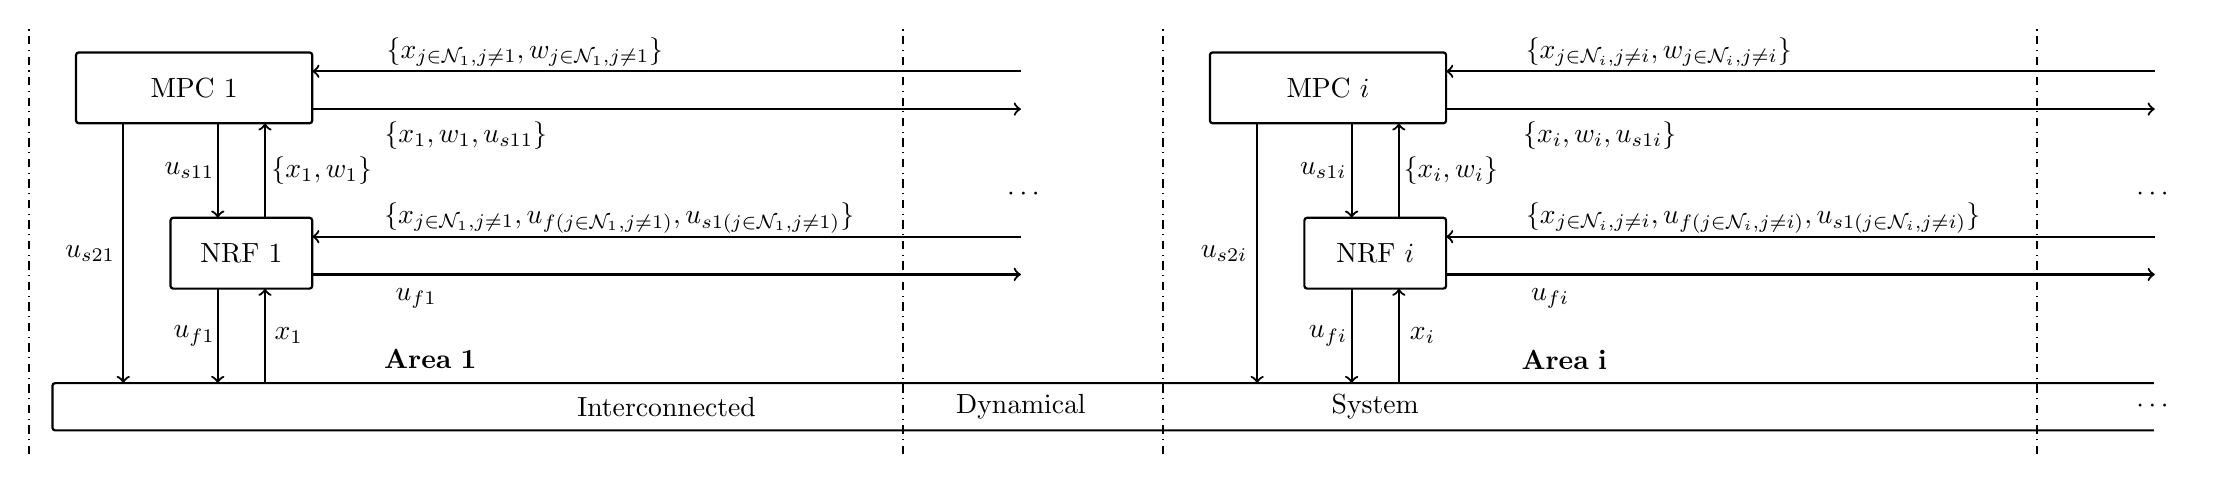
\begin{tikzpicture}[scale=0.6]
				\draw [thick,rounded corners=1]  (-15,-0.5) rectangle +(45,1);
				\draw [thick]  (-2,0)   node {Interconnected};
				\draw [thick]  (5.5,0)   node {Dynamical};
				\draw [thick]  (13,0)   node {System};
				
				\draw [thick,rounded corners=1]  (-1.5-11,2.5) rectangle +(3,1.5);
				\draw [thick]  (0-11,3.25)   node {NRF $1$};
				\node at (4-11,1) {\textbf{Area} $\mathbf 1$};
				\draw [thick,rounded corners=1]  (-3.5-11,6) rectangle +(5,1.5);
				\draw [thick]  (-1-11,6.75)   node {MPC $1$};
				\draw[->,thick] (0.5-11,0.5)--(0.5-11,2.5);
				\node at (1-11,1.5) {$x_1$};
				\draw[->,thick] (-0.5-11,2.5)--(-0.5-11,0.5);
				\node at (-1-11,1.5) {$u_{f1}$};
				\draw[->,thick] (0.5-11,4)--(0.5-11,6);
				\node at (1.7-11,5) {$\{x_1,w_1\}$};
				\draw[->,thick] (-0.5-11,6)--(-0.5-11,4);
				\node at (-1.1-11,5) {$u_{s11}$};
				\draw[->,thick] (-2.5-11,6)--(-2.5-11,0.5);
				\node at (-3.2-11,3.25) {$u_{s21}$};
				\draw[->,thick] (1.5-11,2.8)--(16.5-11,2.8);
				\node at (3.7-11,2.3) {$u_{f1}$};
				\draw[->,thick] (16.5-11,3.6)--(1.5-11,3.6);
				\node at (8-11,4) {$\{x_{j\in\mathcal{N}_1,j\neq 1},u_{f(j\in\mathcal{N}_1,j\neq 1)},u_{s1(j\in\mathcal{N}_1,j\neq 1)}\}$};
				\draw[->,thick] (1.5-11,6.3)--(16.5-11,6.3);
				\node at (4.75-11,5.75) {$\{x_1,w_1,u_{s11}\}$};
				\draw[->,thick] (16.5-11,7.1)--(1.5-11,7.1);
				\node at (6-11,7.5) {$\{x_{j\in\mathcal{N}_1,j\neq 1},w_{j\in\mathcal{N}_1,j\neq 1}\}$};
				\draw[dash dot,thick] (-4.5-11,-1)--(-4.5-11,8);
				\draw[dash dot,thick] (14-11,-1)--(14-11,8);
				
				\node at (5.6,4.5) {$\cdots$};
				
				\draw [thick,rounded corners=1]  (-1.5+13,2.5) rectangle +(3,1.5);
				\draw [thick]  (0+13,3.25)   node {NRF $i$};
				\node at (4+13,1) {\textbf{Area} $\mathbf i$};
				\draw [thick,rounded corners=1]  (-3.5+13,6) rectangle +(5,1.5);
				\draw [thick]  (-1+13,6.75)   node {MPC $i$};
				\draw[->,thick] (0.5+13,0.5)--(0.5+13,2.5);
				\node at (1+13,1.5) {$x_i$};
				\draw[->,thick] (-0.5+13,2.5)--(-0.5+13,0.5);
				\node at (-1+13,1.5) {$u_{fi}$};
				\draw[->,thick] (0.5+13,4)--(0.5+13,6);
				\node at (1.6+13,5) {$\{x_i,w_i\}$};
				\draw[->,thick] (-0.5+13,6)--(-0.5+13,4);
				\node at (-1.1+13,5) {$u_{s1i}$};
				\draw[->,thick] (-2.5+13,6)--(-2.5+13,0.5);
				\node at (-3.2+13,3.25) {$u_{s2i}$};
				\draw[->,thick] (1.5+13,2.8)--(16.5+13,2.8);
				\node at (3.7+13,2.3) {$u_{fi}$};
				\draw[->,thick] (16.5+13,3.6)--(1.5+13,3.6);
				\node at (8+13,4) {$\{x_{j\in\mathcal{N}_i,j\neq i},u_{f(j\in\mathcal{N}_i,j\neq i)},u_{s1(j\in\mathcal{N}_i,j\neq i)}\}$};
				\draw[->,thick] (1.5+13,6.3)--(16.5+13,6.3);
				\node at (4.75+13,5.75) {$\{x_i,w_i,u_{s1i}\}$};
				\draw[->,thick] (16.5+13,7.1)--(1.5+13,7.1);
				\node at (6+13,7.5) {$\{x_{j\in\mathcal{N}_i,j\neq i},w_{j\in\mathcal{N}_i,j\neq i}\}$};
				\draw[dash dot,thick] (-4.5+13,-1)--(-4.5+13,8);
				\draw[dash dot,thick] (14+13,-1)--(14+13,8);
				
				\node at (29.5,4.5) {$\cdots$};
				
				\draw [thick,color=white,fill=white]  (29.5,-0.6) rectangle +(1,1.2);
				
				\node at (29.5,0) {$\cdots$};
		\end{tikzpicture}}
		\caption{High-level implementation scheme depicting the proposed distributed control strategy}\vspace{-1mm}
		\label{fig:scheme}
		\hrulefill\vspace{-2mm}
	\end{figure*}
	
	
	\subsection{Distributed Networks}
	\label{subsec:distrib_part}\vspace{-3mm}
	
	Given that our overarching objective is to control the state evolution of the system under full state measurement availability, the type of networks our procedure is catered towards are described by a more particular class of realizations than the ones from \eqref{eq:ss_a}-\eqref{eq:ss_b}, namely\vspace{-1mm}
	\begin{subequations}
		\begin{align}
			x[k+1] =&\ Ax[k]+B_u u[k]+B_d\,d[k],\label{eq:net_ss_a}\\
			y[k]=&\ \phantom{A}x[k]\label{eq:net_ss_b}.
		\end{align}
	\end{subequations}
	Although we consider that $x$ and $u$ are completely accessible to us, in terms of measurement and actuation respectively, we do not assume that manipulating \emph{all} of this variables is possible from any one location in our physical network. Indeed, a particular feature of distributed networks is the fact that its controlled inputs and measurable state variables are often spatially distributed. This naturally separates the network into a number of $N\in\mathbb{N}$ distinct areas, with $N>1$.\vspace{-3mm}
	
	To each of the network's $N$ areas we now assign two sets of indices, which denote the entries of $x$ and $u$ that are (uniquely) accessible for measurement or actuation in that area. Without loss of generality, we assume that these indices are assigned to the sets in ascending order, since the rows and columns of the matrices expressed in \eqref{eq:net_ss_a}-\eqref{eq:net_ss_b} may be permuted at will. Therefore, each area will be represented by the pair\vspace{-1mm}
	\begin{equation}\label{eq:trip}
		\mathcal{A}_i:=(\mathcal{A}_{xi},\mathcal{A}_{ui}),\,\forall\,i\in\{1:N\},\vspace{-1mm}
	\end{equation}
	which collects the two aforementioned index sets.\vspace{-3mm}
	
	To streamline the definition of the sets given in \eqref{eq:trip}, we will provide generic expressions via the placeholder subscript $\bullet$, which stands for one of the subscripts $\{x,u\}$. Let each set contain a number of $n_{\bullet i}\in\mathbb{N}$ indices, where $n_{\bullet i}>0,\,\forall\,i\in\{1:N\}$, such that we define\vspace{-1mm}
	\begin{equation}\label{eq:net_part}
		\hspace{-1mm}\left\{\begin{split}
			\mathcal{A}_{\bullet i}:=\{\alpha_{\bullet i}+j\ \vert\ j\in1:n_{\bullet i}\},\,\forall\,i\in\{1:N\},\\
			\alpha_{\bullet 1}:=0,\, \alpha_{\bullet \ell}:=\alpha_{\bullet (\ell-1)}+n_{\bullet (\ell-1)},\,\forall\,\ell\in\{2:N\}.
		\end{split}\right.\vspace{-1mm}
	\end{equation}
	To each partition\footnote{As an example, a network with 12 states and 7 inputs could be partitioned as in \eqref{eq:trip}-\eqref{eq:net_part} via the following collection of sets $\scriptsize\begin{array}{l}
			\{(\{1:2\},\{1\}),(\{3:5\},\{2:3\}),(\{6:11\},\{4:5\}),(\{12\},\{6:7\})\}
		\end{array}$} in \eqref{eq:net_part}, we attach the selection matrix\vspace{-1mm}
	\begin{equation}\label{eq:sel_mat}
		S_{\bullet i}:=\left[\begin{array}{ccc}
			e_{\alpha_{\bullet i}+1}&\dots&e_{\alpha_{\bullet i}+n_{\bullet i}}
		\end{array}\right],\,\forall\,i\in\{1:N\},\vspace{-1mm}
	\end{equation}
	with which we define $x_i[k]:=S^\top_{{xi}}x[k]$, $x_{c{i}}:=S^\top_{{xi}}x_c$ and $u_i[k]:=S^\top_{{ui}}u[k]$. Once the network is partitioned, the design of our control scheme can begin.
	
	\section{The Control Architecture}\label{sec:arch}\vspace{-3mm}
	
	\subsection{Global Perspective and Objectives}\label{subsec:global_arch}\vspace{-3mm}
	
	The aim of this paper and of its companion paper \cite{part2} is to formalize the design framework of the two-layer control architecture for the interconnected dynamical system depicted in Figure~\ref{fig:scheme}. By identifying the subset of areas $\mathcal{N}_i\subseteq\{1:N\}$ which are able to transmit information to the network's $i^\text{th}$ area (and which trivially satisfy $i\in\mathcal{N}_i$), for all $i\in\{1:N\}$, the communication graph is clearly designated and the fundamental operating principle of our control scheme is the following:\vspace{-3mm}
	\begin{enumerate}
		\item[$a)$] the state-space implemented NRF subcontrollers receive network state information along with the command signals of other first layer subcontrollers from their areas' neighbourhoods, and use these values to compute the signals denoted $u_{fi}$ in Figure~\ref{fig:scheme};\smallskip
		
		\item[$b)$] the MPC subcontrollers also receive network state information along with the state variables of the NRF subcontroller implementations, denoted $w_i$ in Figure~\ref{fig:scheme}, from their areas' neighbours to compute:\smallskip
		
		\begin{enumerate}
			\item[$b1)$] the command signals denoted by $u_{s1i}$ in Figure~\ref{fig:scheme}, which \emph{are broadcast} and combined additively with the state vectors $x_i$, before the later are fed to the NRF subcontrollers;\smallskip
			
			\item[$b2)$] the command signals denoted by $u_{s2i}$ in Figure~\ref{fig:scheme}, which \emph{remain local} and are combined additively with the NRF outputs $u_{fi}$, to obtain the control signals being sent to the actuators.\vspace{-3mm}
		\end{enumerate}
	\end{enumerate}
	
	\begin{remark}
		In terms of control architecture design, it should be clear that both the first and the second layer employ feedback and feedforward components. However, their goals and their communication-based mechanisms are completely different. Where the first layer focuses on dynamical decoupling and disturbance rejection, the second layer concerns itself with constraint satisfaction and feasibility, in terms of robust control invariance.\vspace{-3mm}
	\end{remark}
	
	Since the MPC layer is built upon the closed-loop interconnection between the NRF layer and the network, it is natural to commence our discussion with the architecture and the requirements of the first layer, along with the way in which the latter interfaces with the network. Therefore, we defer all procedural discussions regarding the second layer (such as the standalone design procedure and the way in which the latter interfaces with the NRF subcontrollers) to our companion paper \cite{part2}.\vspace{-3mm}
	
	\begin{figure}[t]
		\centering
		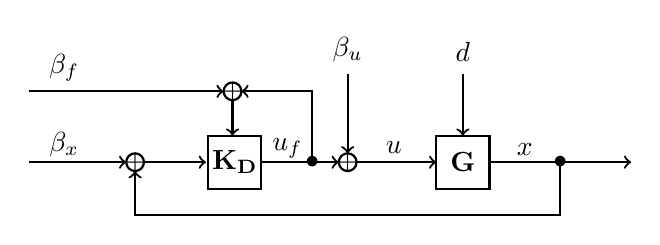
\begin{tikzpicture}[scale=0.225]
			\draw [thick] [->] (-2,0) -- (3.5,0);
			\draw [thick]  (4,0) circle(0.5);
			\draw [thick]  (4,0) node {$+$};
			\draw [thick] (3,1)   node {\bf{ }} (0,1) node {$\beta_x$};
			\draw [thick] [->] (4.5,0) -- (8,0);
			\draw[ thick, xshift=0.1cm]  (8,-1.5) rectangle +(3,3);
			\draw [thick] (9.5,0)   node {{$\,\mathbf{K}_{\mathbf{D}}$}} ;
			\draw [thick] [->] (11.1,0) -- (15.5,0);
			\draw [thick]  (16,0) circle(0.5cm);
			\draw [thick]  (16,0) node {$+$};
			\draw [thick] (12.6,0.8)   node {$u_f$} ;
			\draw [thick] [->] (14,0) -- (14,4)--(10,4);
			\draw [thick] (18.6,0.8)   node {$u$} ;
			\draw [thick] (14,0)   node {$\bullet$} ;
			\draw [thick]  (14.8,0.7)   node {\bf{ }};
			\draw [thick] [->] (16,5) -- (16,0.5);
			\draw [thick]  (0,4)  node[anchor=south] {$\beta_f$};
			\draw [thick]  (9.5,4) circle(0.5);
			\draw [thick]  (9.5,4) node {$+$};
			\draw [thick] [->] (9.5,3.5) -- (9.5,1.5);
			\draw [thick] [->] (-2,4) -- (9,4);
			\draw [thick]  (16,5.1)  node[anchor=south] {$\beta_u$};
			\draw [thick] [->] (16.5,0) -- (21,0);
			\draw [thick]  (21,-1.5) rectangle +(3,3) ;
			\draw [thick]  (22.5,0)   node {{${\bf G}$}} ;
			\draw [thick]  (26,0.7)   node {$x$};
			\draw [thick] [->] (24,0) -- (32,0);
			\draw [thick] (28,0)   node {$\bullet$} ;
			\draw [thick] [->] (28,0) -- (28,-3) -- (4,-3)-- (4, -0.5);
			\draw [thick] [->] (22.5,5) -- (22.5,1.5);
			\draw [thick]  (22.5,5.1)  node[anchor=south] {$d$};
		\end{tikzpicture}
		\caption{Feedback loop of a network's model ${\bf G}(z)$ with the NRF-based implementation $\mathbf{K}_{\bf \mathbf{D}}(z)$}
		\label{fig:NRF_implem}
	\end{figure}
	
	\begin{figure*}
		\begin{equation}\label{eq:area_NRF}\tag{16}
			\mathbf{K}_{\mathbf{D}i}(z)=\left[\scriptsize\begin{array}{c|c}
				A_{wi}-z I_{n_{wi}} & B_{wi} \\ \hline C_{wi} & D_{wi}
			\end{array}\right]:= \left[\tiny\begin{array}{ccc|c}
				A_{r(\alpha_{ui}+1)}-z I_{n_{r(\alpha_{ui}+1)}} & & & B_{r(\alpha_{ui}+1)} \\
				& \ddots & & \vdots \\
				& & A_{r(\alpha_{ui}+n_{ui})}-z I_{n_{r(\alpha_{ui}+n_{ui})}} & B_{r(\alpha_{ui}+n_{ui})} \\ \hline 
				C_{r(\alpha_{ui}+1)} & & & D_{r(\alpha_{ui}+1)}\\
				& \ddots & & \vdots\\
				& & C_{r(\alpha_{ui}+n_{ui})} & D_{r(\alpha_{ui}+n_{ui})}\\
			\end{array}\right].\vspace{1mm}
		\end{equation}
		\hrulefill\vspace{-1mm}
	\end{figure*}
	
	\subsection{Architecture of the NRF Layer}\label{subsec:NRF_arch}\vspace{-3mm}
	
	
	Given some subset of the complex plane $\mathbb{C}_{g}\subseteq\mathbb{C}$ with desirable properties, the control architecture's first layer is based upon a so-called $\mathbb{C}_g$-allocating NRF pair, described in Appendix~\ref{app:aux}. Such a pair is formed by two proper TFMs, $\mathbf{\Phi}\in\mathcal{R}(z)^{n_u\times n_u}$ and $\mathbf{\Gamma}\in\mathcal{R}(z)^{n_u\times n_x}$, and we also refer to Appendix~\ref{app:aux} for details on the pair's structure and computation. Crucially, the NRF-based controllers developed in \cite{NRF} are implemented as in Figure~\ref{fig:NRF_implem}, where the distributed controller is represented by\vspace{-3mm}
	\begin{equation}\label{eq:Kd_def}
		\mathbf{K}_{\mathbf{D}}(z):=\begin{bmatrix}
			\mathbf{\Phi}(z) & \mathbf{\Gamma}(z)
		\end{bmatrix}.\vspace{-3mm}
	\end{equation}
	Alongside the signals introduced in Section~\ref{subsec:sys_nots}, we take into account a number of exogenous signals. These are:\vspace{-3mm}
	\begin{enumerate}
		\item[$a)$] the state-feedback disturbance $\beta_x[k]$, which includes state measurement noise and the $u_{s1i}[k]$ signals discussed in Section~\ref{subsec:global_arch}, along with encoding errors associated with the latter; \smallskip
		
		\item[$b)$] the plant-input disturbance $\beta_u[k]$, which includes the $u_{s2i}[k]$ signals discussed in Section~\ref{subsec:global_arch} and various encoding errors associated with them; \smallskip
		
		\item[$c)$] the NRF-feedforward disturbance $\beta_f[k]$, which arises in the context of the communication between neighbouring first layer subcontrollers.\vspace{-3mm}
	\end{enumerate}
	We concatenate all of these exogenous (with respect to the first layer) signals, along with $d$ from \eqref{eq:net_ss_a}, into the signal vector
	$ d_s[k]:=\begin{bmatrix}
		\beta_{x}^\top[k] & \beta_{u}^\top[k] & \beta_f^\top[k] & d^\top[k]
	\end{bmatrix}^\top$.\vspace{-3mm}
	
	
	
	\begin{remark}\label{rem:com}
		We assume that the communication infrastructure of our control architecture is endowed error-detecting/correcting transmission mechanisms. Therefore, all communication errors affecting transmitted information are modelled as disturbance which originates at the source of transmission, not on the receiving ends.\vspace{-3mm}
	\end{remark}
	
	
	
	\subsection{Objectives of the NRF Layer}\label{subsec:NRF_obj}\vspace{-3mm}
	
	
	
	Although the ultimate goal of our endeavour is represented by a distributed constraint management policy, a "brute force" MPC-based approach may prove \emph{highly conservative}, as a consequence of failing to grasp the structured dynamics of the controlled network. As shown in Figure~\ref{fig:scheme}, the subcontrollers of the second layer do not exchange information regarding the values of the command signals $u_{s1i}[k]$ and $u_{s2i}[k]$. They must, therefore, compensate any cross-coupling induced by the control action of other subcontrollers from their layer, while also being restricted to exchanging information via the network's available communication infrastructure.
	\vspace{-3mm}
	
	All of the aforementioned challenges have to be successfully alleviated by our architecture's first layer, which must simultaneously achieve the following objectives:\vspace{-3mm}
	\begin{enumerate}
		\item[$\mathrm I)$] it must be implementable in a distributed manner, using sparse state-space models that are computationally inexpensive to deploy (Section~\ref{subsec:ss_implems});\smallskip
		
		\item[$\mathrm{II})$] it must render the closed-loop maps of its interconnection as simple expressions, by means of a rich and highly tractable parametrization (Section~\ref{subsec:theo_NRF});\smallskip
		
		\item[$\mathrm{III})$] it must enable the dynamical decoupling of the network areas discussed in Sections~\ref{subsec:distrib_part}~and~\ref{subsec:global_arch}, for the benefit of the MPC layer, through numerically sound procedures available in literature (Section~\ref{sec:NRF_des});\vspace{-3mm}
		
	\end{enumerate}
	
	The remainder of this paper is dedicated to presenting the solutions to these design challenges.\vspace{-3mm}
	
	\section{Theoretical Results}\vspace{-3mm}
	\label{sec:NRF_theo}
	
	\subsection{State-space Implementations for NRF Control}\vspace{-3mm}
	\label{subsec:ss_implems}
	
	The main feature of the NRF framework is the fact that the command signal vector $u_f$ can be computed in a \emph{distributed} manner, by enforcing an appropriate sparsity structures upon the controller's NRF pair (see \cite{NRF}).\vspace{-3mm}
	
	For the particular setting described in Section~\ref{subsec:distrib_part}, in which the network is partitioned into $N$ distinct areas as in \eqref{eq:net_part}, it is possible to employ the TFM from \eqref{eq:Kd_def} in order to \emph{independently} compute\vspace{-3mm}
	\begin{equation}\label{eq:uf_implem}
		\hspace{-1mm}u_{fi}[k]:=S_{ui}^\top u_f[k] = \mathbf{K}_{\mathbf{D}i}(z)\star\scriptsize\begin{bmatrix}
			u_f[k]+\beta_f[k] \\ x[k]+\beta_{x}[k]
		\end{bmatrix},\normalsize\vspace{-2mm}
	\end{equation}
	for all $i\in\{1:N\}$, with the TFMs $\mathbf{K}_{\mathbf{D}i}(z):=S_{ui}^\top\mathbf{K}_{\mathbf{D}}(z)$ denoting each area's NRF-based subcontroller. Although the subcontrollers $\mathbf{K}_{\mathbf{D}i}(z)$ from \eqref{eq:uf_implem} can always be implemented \emph{separately} in the control scheme from Figure~\ref{fig:NRF_implem}, this does not immediately lead to tractable formulations for distributed constraint management.\newpage
	
	In order to be effective, these subcontrollers must be accompanied by state-space representation which mirror the sparsity patterns of their TFMs. The next constructive result addresses precisely this issue.\vspace{-3mm}
	
	\begin{proposition}\label{prop:ss_implem}
		Let the rows of the TFM from \eqref{eq:Kd_def} be described by the \emph{minimal} realizations\vspace{-3mm}
		\begin{equation}\label{eq:Kd_rows}
			\mathrm{row}_\ell\left(\mathbf{K}_{\mathbf{D}}(z)\right)=\left[\scriptsize \begin{array}{c|c}
				\widehat A_{\ell}-z I_{n_{r\ell}} & \widehat B_{\ell} \\ \hline \widehat C_{\ell} & \widehat D_{\ell}
			\end{array}\right], \forall\, \ell\in\{1:n_u\},\vspace{-3mm}
		\end{equation}for which we define the polynomials\vspace{-2mm}
		\begin{equation}\label{eq:min_poly}
			\hspace{-1mm}\chi_\ell(z):=\det(zI_{n_{r\ell}}-\widehat A_{\ell})=z^{n_{r\ell}}+\sum_{j=1}^{n_{r\ell}}a_{j\ell}z^{(n_{r\ell}-j)}.\hspace{-1mm}\vspace{-3mm}
		\end{equation}
		Then, by expressing the aforementioned row TFMs as\vspace{-3mm}
		\begin{equation}\label{eq:TFM_coefs}
			\mathrm{row}_\ell\left(\mathbf{K}_{\mathbf{D}}(z)\right)=\widehat D_{\ell}+\frac{1}{\chi_\ell(z)}\sum_{j=1}^{n_{r\ell}}K_{j \ell} z^{(n_{r\ell}-j)},\vspace{-3mm}
		\end{equation}
		we have that:
		\begin{enumerate}
			\item[$i)$] The following identities hold\vspace{-3mm}
			\begin{equation}\label{eq:Kd_implem}
				\mathrm{row}_\ell\left(\mathbf{K}_{\mathbf{D}}(z)\right)=\left[\scriptsize\begin{array}{c|c}
					A_{r\ell}-z I_{n_{r\ell}} & B_{r\ell} \\ \hline C_{r\ell} & D_{r\ell}
				\end{array}\right],\vspace{-3mm}
			\end{equation}
			for all $\ell\in\{1:n_u\}$, where\vspace{-3mm}
			\begin{equation}\label{eq:mat_coef}
				\left\{\begin{split}
					\widetilde{A}_{r\ell}:=&\ \scriptsize\begin{bmatrix}
						-a_{1\ell} &\dots& -a_{(n_{r\ell}-1)\ell}
					\end{bmatrix}^\top,\\ A_{r\ell}:=&\ \scriptsize\begin{bmatrix}
						\widetilde{A}_{r\ell} & I_{n_{r\ell}-1}\\
						-a_{n_{r\ell}\ell} & O
					\end{bmatrix},\\
					\ B_{r\ell}:=&\ \scriptsize\begin{bmatrix}
						K_{1i}^\top &\dots& K_{n_{r\ell}i}^\top
					\end{bmatrix}^\top,\\ C_{r\ell}:=&\ \scriptsize\begin{bmatrix}
						1 & 0 & \dots & 0
					\end{bmatrix},\\
					D_{r\ell}:=&\ \widehat D_{\ell}=\lim_{|z|\rightarrow\infty}\mathrm{row}_\ell\left(\mathbf{K}_{\mathbf{D}}(z)\right);
				\end{split}\right.\vspace{-3mm}
			\end{equation}
			
			\item[$ii)$] The realizations given in \eqref{eq:Kd_implem} are \emph{minimal};\smallskip
			
			\item[$iii)$] The columns of $B_{r\ell}$ and $D_{r\ell}$ have \emph{the same sparsity structure} as $\mathrm{row}_\ell\left(\mathbf{K}_{\mathbf{D}}(z)\right)$, which is to say that\vspace{-3mm}
			\begin{equation}
				\mathrm{elm}_{\ell j}\left(\mathbf{K}_{\mathbf{D}}(z)\right) \equiv 0 \Longrightarrow \left\{\begin{array}{l}
					\mathrm{col}_{j}(B_{r\ell}) = O,\\
					\mathrm{col}_{j}(D_{r\ell}) = 0,
				\end{array}\right.\vspace{-3mm}
			\end{equation}
			for all $j\in\{1:n_x+n_u\}$;\smallskip
			
			\item[$iv)$] The subcontrollers $\mathbf{K}_{\mathbf{D}i}(z)$ can be implemented, for all $i\in\{1:N\}$, via the structured realizations given in \eqref{eq:area_NRF}, which are located at the top of the page.\vspace{-5mm}
		\end{enumerate}
	\end{proposition}
	\begin{pf}
		See Appendix~\ref{app:proofs}.
	\end{pf}
	
	\begin{figure*}
		\begin{subequations}
			\begin{align}\label{eq:F_Q}\tag{17a}
				&\ \mathbf{F}_{\mathbf{Q}}(z):=\left[\begin{array}{c:c:c:c}
					\mathbf{N}(z)\widetilde{\mathbf{X}}_{\mathbf{Q}}(z) &
					\mathbf{N}(z)\widetilde{\mathbf{Y}}_{\mathbf{Q}}(z) &
					\mathbf{N}(z)\left(\widetilde{\mathbf{Y}}_{\mathbf{Q}}^{\mathrm{diag}}(z)-\widetilde{\mathbf{Y}}_{\mathbf{Q}}(z)\right) & 
					(\mathbf{N}(z)\widetilde{\mathbf{X}}_{\mathbf{Q}}(z)+I_{n_x})\mathbf{G}_d(z)\\\hdashline
					\mathbf{M}(z)\widetilde{\mathbf{X}}_{\mathbf{Q}}(z) &
					\mathbf{M}(z)\widetilde{\mathbf{Y}}_{\mathbf{Q}}(z)-I_{n_u} &
					\mathbf{M}(z)\left(\widetilde{\mathbf{Y}}_{\mathbf{Q}}^{\mathrm{diag}}(z)-\widetilde{\mathbf{Y}}_{\mathbf{Q}}(z)\right) & 
					\mathbf{M}(z)\widetilde{\mathbf{X}}_{\mathbf{Q}}(z)\mathbf{G}_d(z)
				\end{array}\right],\\
				\label{eq:I_Q}\tag{17b}
				&\begin{array}{ll}
					\ \mathbf{I}_{\mathbf{Q}}(z):=\left[\begin{array}{c:c}
						\mathbf{Y}(z)\mathbf{J}_1(z)+\mathbf{N}(z)\mathbf{Q}(z)\mathbf{J}_1(z)&\mathbf{N}(z)\mathbf{J}_2(z)\\\hdashline
						\mathbf{X}(z)\mathbf{J}_1(z)+\mathbf{M}(z)\mathbf{Q}(z)\mathbf{J}_1(z)&\mathbf{M}(z)\mathbf{J}_2(z)
					\end{array}\right],&\begin{array}{l}
						\mathbf{J}_1(z):=\widetilde{\mathbf{M}}(z)(zI_{n_x}-A)^{-1}z,\\
						\mathbf{J}_2(z):=\widetilde{\mathbf{Y}}_{\mathbf{Q}}^{\mathrm{diag}}(z)C_w(zI_{n_w}-A_w)^{-1}z.
					\end{array}
				\end{array}
			\end{align}
		\end{subequations}
		\hrulefill
	\end{figure*}
	
	\begin{remark}\label{rem:sparse_real}
		The polynomials $\chi_\ell(z)$ can be computed in a numerically reliable manner by first effecting a change of coordinates in the realization from \eqref{eq:Kd_implem} which brings $\widehat{A}_\ell$ to Real Schur Form. This representation can then be used to also compute the constant real row vectors $K_{j\ell}$.\vspace{-3mm}
	\end{remark}
	
	The realizations given in \eqref{eq:area_NRF} are precisely the sought-after representations mentioned in objective $\mathrm I)$ from Section~\ref{subsec:NRF_obj}, and we point out that the particular structure of the matrices expressed in \eqref{eq:mat_coef} plays a key role in facilitating the design of a MPC-based second layer (see our companion paper \cite{part2} for more details).\vspace{-3mm}
	
	It now becomes relevant to investigate the expressions of the closed-loop maps obtained by implementing the state-space-based subcontrollers from \eqref{eq:area_NRF}. Before doing so, however, we must introduce some additional notation. We denote the orders of the aforementioned realizations as $n_{wi}:=\textstyle\sum_{\ell=1}^{n_{ui}} n_{r\ell}$ and let $n_w:=\textstyle\sum_{i=1}^N n_{wi}$. Additionally, we denote the initial conditions of the subcontrollers given in \eqref{eq:area_NRF} as $w_{ci}\in\mathbb{R}^{n_{wi}},\,\forall\,i\in\{1:N\}$ and we define $w_c:=\begin{bmatrix}
		w_{c1}^\top&\dots&w_{cN}^\top
	\end{bmatrix}^\top$. With this notation at hand, we may now tackle objective $\mathrm{II})$ from Section~\ref{subsec:NRF_obj}.\vspace{-3mm}
	
	
	\subsection{Theoretical Guarantees of NRF-based Control}\label{subsec:theo_NRF}\vspace{-3mm}
	
	Yet another benefit of NRF-based control is the fact that, even in the distributed setting, \emph{all} closed-loop maps from exogenous disturbance \emph{and} initial conditions depend upon a freely tunable parameter (see Appendix~\ref{app:aux}). This flexibility is showcased through the following result, which offers the theoretical framework for the \emph{complete} tuning of closed-loop response presented in the sequel. \vspace{-3mm}
	
	\begin{theorem}\label{thm:NRF_state}
		Let $\mathbb{C}_g\subseteq\mathbb{C}$ and let $\mathbb{C}_b:=\mathbb{C}\backslash\mathbb{C}_g$. Let a network described by \eqref{eq:ss_a}-\eqref{eq:ss_b} be split into a number of $N$ areas, as in \eqref{eq:trip}-\eqref{eq:net_part}, and let it be connected, as in Figure~\ref{fig:NRF_implem}, to a set of NRF subcontrollers of type \eqref{eq:uf_implem}. Assume that:
		\begin{enumerate}
			\item[A1)] The subrealization $(A,B_u,I_{n_x},O)$ from \eqref{eq:net_ss_a}-\eqref{eq:net_ss_b} is $\mathbb{C}_b$-controllable;\medskip
			
			\item[A2)] The collection $(\mathbf{N}(z),\mathbf{M}(z),\mathbf{X}(z),\mathbf{Y}(z),\widetilde{\mathbf{N}}(z),\widetilde{\mathbf{M}}(z),$ $\widetilde{\mathbf{X}}(z),\widetilde{\mathbf{Y}}(z))$ is a doubly coprime factorization over $\mathbb{C}_g$ of $\mathbf{G}_u(z):=(z I_{n_x}-A)^{-1}B_u$, as in Appendix~\ref{app:aux};\medskip
			
			\item[A3)] The pair $(\mathbf{\Phi},\mathbf{\Gamma})$ is a $\mathbb{C}_g$-allocating NRF pair (see Appendix~\ref{app:aux}), based upon the aforementioned factorization of $\mathbf{G}_u(z)$;\medskip
			
			\item[A4)] The control laws from \eqref{eq:uf_implem} are based upon $(\mathbf{\Phi},\mathbf{\Gamma})$, and are implemented via the realizations given in \eqref{eq:area_NRF};\vspace{-3mm}
		\end{enumerate}
		Then, by using \eqref{eq:area_NRF} to define $A_w:=\mathrm{diag}(A_{w1},\dots,A_{wN})$ along with $C_w:=\mathrm{diag}(C_{w1},\dots,C_{wN})$, the closed-loop dynamics of the network's states and the NRF subcontrollers' outputs in Figure~\ref{fig:NRF_implem} are given by\stepcounter{equation}\vspace{-3mm}
		\begin{equation}\label{eq:cl_dyn}
			\begin{bmatrix}
				x[k]  \\  u_f[k]
			\end{bmatrix}=\mathbf{F}_{\mathbf{Q}}(z)\star d_s[k]+\mathcal{I}_{\mathbf{Q}}[k]
			{\begin{bmatrix}
					x_c \\  w_c
			\end{bmatrix}}
			\,,\vspace{-3mm}
		\end{equation}
		where we have that:\vspace{-3mm}
		\begin{enumerate}
			\item[$i)$] The TFM denoted $\mathbf{F}_{\mathbf{Q}}(z)$ is expressed in \eqref{eq:F_Q} at the top of this page, with $\widetilde{\mathbf{Y}}_{\mathbf{Q}}(z)$, $\widetilde{\mathbf{Y}}_{\mathbf{Q}}(z)$ and $\widetilde{\mathbf{Y}}_{\mathbf{Q}}^{\mathrm{diag}}(z)$ being defined in \eqref{eq:aux_NRF} within Appendix~\ref{app:aux}, and where\vspace{-3mm}
			\begin{equation*}
				\mathbf{G}_d(z):=(z I_{n_x}-A)^{-1}B_d;\vspace{-3mm}
			\end{equation*}
			
			\item[$ii)$] The matrix $\mathcal{I}_{\mathbf{Q}}[k]$ is the inverse $\mathcal{Z}$-transform of the TFM defined in \eqref{eq:I_Q} at the top of this page;\smallskip
			
			
			\item[$iii)$] The TFM $\mathbf{Q}(z)$ appearing in \eqref{eq:F_Q}-\eqref{eq:I_Q} is the $\mathbf{Q}$-parameter which designates the employed NRF pair;\smallskip
			
			\item[$iv)$] All the TFMs defined in \eqref{eq:F_Q}-\eqref{eq:I_Q} are proper and $\mathbb{C}_b$-bounded.\vspace{-7mm}
		\end{enumerate}
	\end{theorem}
	
	\begin{pf}
		See Appendix~\ref{app:proofs}.\vspace{-3mm}
	\end{pf}
	
	\begin{remark}
		We highlight the fact that assumptions A1) through A4) in Theorem~\ref{thm:NRF_state} are \emph{in no way restrictive}, from a practical standpoint. The closed-loop dynamics of the network cannot be tuned with respect to $\mathbb{C}_g$ unless A1) holds, while the factorization and the NRF pair from assumptions A2) through A4) can be reliably obtained via classical system-theoretical results (see \cite{NRF} and \cite{aug_sparse}).\vspace{-3mm}
	\end{remark}
	
	By inspecting the expressions obtained in \eqref{eq:F_Q}-\eqref{eq:I_Q}, it becomes clear that the distributed implementations proposed in Proposition~\ref{prop:ss_implem} fully address objective $\mathrm{II})$ from Section~\ref{subsec:NRF_obj}. Indeed, the $\mathbf{Q}$-parameter which characterizes all of these expressions represents the \emph{main tuning parameter} of our control architecture's first layer, and the freedom in choosing it provides fertile grounds for the development of NRF-based design procedures. This endeavour represents the focus of our next section, in which we tackle the final objective stated in Section~\ref{subsec:NRF_obj}.
	
	\vspace{-3mm}
	
	\begin{remark}
		Since the NRF pair used in Theorem~\ref{thm:NRF_state} is $\mathbb{C}_g$-allocating, then its corresponding $\mathbf{Q}$-parameter \emph{must} be $\mathbb{C}_b$-bounded (see Appendix~\ref{app:aux} and \cite{NRF}), which constitutes the only real restriction placed upon $\mathbf{Q}(z)$. We also point out that certain choices of $\,\mathbb{C}_g$ are preferable, from a practical point of view. For example, by choosing $\,\mathbb{C}_g\subseteq\mathbb{S}$, it follows (see Appendix~\ref{app:aux}) that the the state variables of the plant and those of the NRF subcontrollers will be bounded at all times, for any initial conditions of these systems and for any bounded exogenous signals.\vspace{-3mm}
	\end{remark}
	
	
	\section{NRF Layer Design}\vspace{-3mm}
	\label{sec:NRF_des}
	
	\subsection{The Decoupling-based Approach}\vspace{-3mm}\label{subsec:decup}
	
	In order to formulate the design procedure of our architecture's first layer, we need to account for the state variables of the implementations from \eqref{eq:area_NRF}. Thus, aside from the $x$ and $u$ subscripts appearing in \eqref{eq:net_part}-\eqref{eq:sel_mat}, we introduce the additional subscript $w$, in order to refer to the state vector of each area's NRF subcontroller, and we extend the index collection defined originally in \eqref{eq:trip} to $\mathcal{A}_i:=(\mathcal{A}_{xi},\mathcal{A}_{ui},\mathcal{A}_{wi}),\,\forall\,i\in\{1:N\}$.\vspace{-3mm} 
	
	We may now rewrite the closed-loop dynamics obtained in Theorem~\ref{thm:NRF_state} and then partition them into the network areas discussed in Section~\ref{subsec:distrib_part}.	As previously mentioned in Section~\ref{subsec:NRF_arch}, the MPC commands $u_{s1i}[k]$ and $u_{s2i}[k]$, depicted in Figure~\ref{fig:scheme}, are folded into $\beta_x[k]$ and $\beta_u[k]$. Thus, we will refer to the following quadruplet $\{S_{xi}^\top\beta_x^{}[k],S_{ui}^\top\beta_u^{}[k],x_{ci},w_{ci}\}$ as the \emph{$i^\text{th}$ area's variables}, from the point of view of that area's local MPC.\vspace{-3mm}
	
	All of these new terms enable us to express the dynamics of the $i^\text{th}$ area as a combination between the effect of exogenous disturbance, given by a TFM's input-output response in \eqref{eq:io_resp}, and that of area cross-coupling, given by\vspace{-3mm}
	\begin{equation}\label{eq:dyn_i}
		\hspace{-1mm}\scriptsize\begin{bmatrix}
			x_i[k] \\  u_{fi}[k]
		\end{bmatrix}= Z_i^\top\mathbf{F}_{\mathbf{Q}}(z)\scriptsize\begin{bmatrix}
			O \\  I_{(n_u+n_d)}
		\end{bmatrix}\star \scriptsize\begin{bmatrix}
			\beta_f[k] \\ d[k]
		\end{bmatrix} + \sum_{j=1}^N\mathcal{E}_{ij}[k],\normalsize\vspace{1mm}
	\end{equation}
	where $Z_i:=\mathrm{diag}(S_{xi},S_{ui})$. Moreover, the cross-coupling may be represented as the input-output response of another TFM and a free response term which depends upon the initial conditions of the coupled area, thus yielding\vspace{-3mm}
	\begin{equation}\label{eq:Ei_def}
		\hspace{-1mm}\mathcal{E}_{ij}[k]:= Z_i^\top\mathbf{F}_{\mathbf{Q}}(z)\hspace{-1mm}\tiny\begin{bmatrix}
			Z_j\\O
		\end{bmatrix}\star \tiny\begin{bmatrix}
			S_{xj}^\top\beta_x[k]\\S_{uj}^\top\beta_u[k]
		\end{bmatrix}\hspace{-1mm} + Z_i^\top \mathcal{I}_{\mathbf{Q}}[k]{Z}_{cj}\hspace{-1mm}\tiny\begin{bmatrix}
			x_{cj}\\w_{cj}
		\end{bmatrix},\normalsize\hspace{-2mm}\vspace{1mm}
	\end{equation}
	which is the \emph{effect} of the $j^\text{th}$ area's variables on the $i^\text{th}$ area, and in which  the time-domain expression from the right-hand term depends upon ${Z}_{ci}:=\mathrm{diag}(S_{xi},S_{wi})$.\vspace{-3mm}
	
	\begin{remark}
		The particular formulations obtained in this section facilitate the construction of the prediction models, which are then employed in the distributed synthesis of our top layer constraint management policies.\vspace{-3mm}
	\end{remark}
	
	In light of \eqref{eq:dyn_i}-\eqref{eq:Ei_def}, the final objective of the NRF layer, meant to facilitate the second layer's implementation, now becomes apparent. With respect to the communication neighbourhoods introduced in Section~\ref{subsec:global_arch}, the $i^\text{th}$ area's NRF subcontroller must:\vspace{-3mm}
	\begin{enumerate}
		\item[$a)$] only employ information originating in $\mathcal{N}_i$;\smallskip
		\item[$b)$] handle the effect of $\beta_f[k]$ and $d[k]$ according to some pre-specified design objective.\smallskip
		\item[$c)$] minimize the effect of $S_{xj}^\top\beta_x^{}[k]$ and of $S_{uj}^\top\beta_u^{}[k],$ for all indices $j\in\{1:N\}\backslash\{i\}$;\smallskip
		\item[$d)$] minimize the effect of $x_{cj}$ and of $w_{cj},$ for all indices $j\in\{1:N\}\backslash\mathcal{N}_i$.\vspace{-3mm}
	\end{enumerate}
	
	We now proceed to formalize all of these requirements.
	
	\begin{figure*}
		\begin{equation}\label{eq:MM_prob}\tag{27}
			\begin{split}
				&\min\limits_{\mathbf{Q}(z),\gamma_{di},\gamma_{u{ij}},\gamma_{c{ij}}} \textstyle\sum_{i=1}^N\bigg(\tau_{di}\gamma_{di} + \textstyle\sum_{j=1}^N(\tau_{u{ij}}\gamma_{u{ij}}+\tau_{c{ij}}\gamma_{c{ij}})\bigg),\\
				&\text{subject to }
				\left\{\begin{split}
					&\text{\eqref{eq:con_NRF_a}-\eqref{eq:con_NRF_b}, \eqref{eq:con_pert}-\eqref{eq:con_init} and \eqref{eq:con_gamma},}\\
					&\mathbf{Q}\in\mathcal{R}(z)^{n_u\times n_x}\text{ strictly proper and }\mathbb{C}_b\text{-bounded}.
				\end{split}\right.
			\end{split}\vspace{-2mm}
		\end{equation}
		\hrulefill\vspace{-2mm}
	\end{figure*}
	
	\subsection{Formulating the Model Matching Problem}\vspace{-3mm}
	
	The most straightforward of the aforementioned requirements is the first one, which places restrictions upon the sparsity structure of the pair $(\mathbf{\Phi}(z),\mathbf{\Gamma}(z))$. This communication constraint is formalized via the conditions\vspace{-3mm}
	\begin{subequations}
		\begin{align}\label{eq:con_NRF_a}
			\hspace{-1mm}S_{ui}^\top\mathbf{\Phi}(z)S_{{uj}}\equiv&\ O,\forall\,i\in\{1:N\},\, j\in\{1:N\}\backslash\,\mathcal{N}_i,\\
			S_{ui}^\top\mathbf{\Gamma}(z)S_{{xj}}\equiv&\ O,\forall\,i\in\{1:N\},\, j\in\{1:N\}\backslash\,\mathcal{N}_i,\label{eq:con_NRF_b}
		\end{align}
	\end{subequations}
	\phantom{ }\vspace{-10mm}
	
	which form an \emph{exact model matching problem} (see \cite{aug_sparse}). \vspace{-3mm}
	
	The last three requirements stated in Section~\ref{subsec:decup} can be tackled by first selecting, for each area of the network, a triplet of TFMs which describes its closed-loop response. These separate naturally into those which concern the exogenous disturbance vectors $\beta_f[k]$ and $d[k]$, namely\vspace{-3mm}
	\begin{subequations}
		\begin{align}\label{eq:des_d_a}
			&\mathbf{T}_{di}\in\mathcal{R}(z)^{(n_{xi}+n_{ui})\times(n_u+n_d)},\,\forall\,i\in\{1:N\},\\
			&\mathbf{T}_{di}(z)\text{ proper and $\mathbb{C}_b$-bounded},\,\forall\,i\in\{1:N\},\label{eq:des_d_b}
		\end{align}
	\end{subequations}
	\phantom{ }\vspace{-11mm}
	
	those concerning the disturbance channels associated with the command signals computed by the MPC layer\vspace{-3mm}
	\begin{subequations}
		\begin{align}\label{eq:des_u_a}
			&\mathbf{T}_{ui}\in\mathcal{R}(z)^{(n_{xi}+n_{ui})\times (n_x+n_u)},\,\forall\,i\in\{1:N\},\\\label{eq:des_u_b}
			&\mathbf{T}_{ui}(z)\text{ proper and $\mathbb{C}_b$-bounded},\,\forall\,i\in\{1:N\},\\\label{eq:des_u_c}
			&\mathbf{T}_{u{ij}}(z):=\mathbf{T}_{ui}(z)Z_i,\,\forall\,i,j\in\{1:N\},\\
			&\mathbf{T}_{u{ij}}(z)\equiv O,\forall\,i\in\{1:N\},\forall\, j\in\{1:N\}\backslash\{i\},\label{eq:des_u_d}
		\end{align}
	\end{subequations}
	\phantom{ }\vspace{-11mm}
	
	and those concerning the initial conditions of the areas\vspace{-3mm}
	\begin{subequations}
		\begin{align}\label{eq:des_c_a}
			&\mathbf{T}_{c{i}}\in\mathcal{R}(z)^{(n_{xi}+n_{ui})\times (n_x+n_w)},\,\forall\,i\in\{1:N\},\\\label{eq:des_c_b}
			&\mathbf{T}_{c{i}}(z)\text{ proper and $\mathbb{C}_b$-bounded},\,\forall\,i\in\{1:N\},\\\label{eq:des_c_c}
			&\mathbf{T}_{c{ij}}(z):=\mathbf{T}_{c{i}}(z){Z}_{cj},\,\forall\,i,j\in\{1:N\},\\
			&\mathbf{T}_{c{ij}}(z)\equiv O,\forall\,i\in\{1:N\},\forall\, j\in\{1:N\}\backslash\,\mathcal{N}_i.\label{eq:des_c_d}
		\end{align}
	\end{subequations}
	\phantom{ }\vspace{-11mm}
	
	
	Once the closed-loop response TFMs are selected, the design problem reduces to minimizing the difference between the TFMs appearing in \eqref{eq:dyn_i}-\eqref{eq:Ei_def} (along with the $\mathcal{Z}$-transforms of the $Z_i^\top \mathcal{I}_{\mathbf{Q}}[k]{Z}_{cj}$ terms) and those from \eqref{eq:des_d_a}-\eqref{eq:des_c_d}, in terms of a suitable system norm.
	\vspace{-3mm}
	
	\begin{remark}\label{rem:H2}
		In order to provide a flexible design framework, we will formulate our model matching expressions in terms of a generic system norm. Certain norms admit particularly tractable formulations for affine expressions of our design parameter $\mathbf{Q}(z)$, which include most of the terms that appear in \eqref{eq:F_Q}-\eqref{eq:I_Q}. A relevant example of this design choice is the $\mathcal{H}_2$-based approach given in \cite{Rotko}.\vspace{-3mm}
	\end{remark}
	
	We introduce scalar upper bounds ${\gamma}_{d{i\phantom{j}}}$, ${\gamma}_{u{ij}}$ and ${\gamma}_{c{ij}}$, where $i,j\in\{1:N\}$, for each individual model matching subproblem such that\vspace{-3mm}
	\begin{subequations}
		\begin{align}\label{eq:con_pert}
			&\hspace{-3mm}\left\|Z_i^\top\mathbf{F}_{\mathbf{Q}}(z)\tiny\hspace{-1mm}\begin{bmatrix}
				O \\  I_{(n_u+n_d)}
			\end{bmatrix}\hspace{-1mm}-\mathbf{T}_{di}(z)\right\|\leq \gamma_{di},\\
			\label{eq:con_cmd}
			&\hspace{-3mm}\left\|Z_i^\top\mathbf{F}_{\mathbf{Q}}(z)\tiny\hspace{-1mm}\begin{bmatrix}
				Z_j\\O
			\end{bmatrix}\hspace{-1mm}-\mathbf{T}_{u{ij}}(z)\right\|\leq \gamma_{u{ij}},\forall\,j\in\{1:N\},\hspace{-2mm}\\
			\label{eq:con_init}
			&\hspace{-3mm}\left\|Z_i^\top\mathbf{I}_{\mathbf{Q}}(z){Z}_{cj}-\mathbf{T}_{c{ij}}(z)\right\|\leq \gamma_{c{ij}},\forall\,j\in\{1:N\},
		\end{align}
	\end{subequations}
	\phantom{ }\vspace{-9mm}
	
	for each area index $i\in\{1:N\}$. As shown in the sequel, the NRF layer design problem boils down to a generic optimization problem, whose aim consists in the simultaneous minimization of all the upper bounds which are located in the right-hand terms of \eqref{eq:con_pert}-\eqref{eq:con_init}.
	
	
	Before moving on to the computational details of our proposed procedure, we point out that our approach showcases a series of important similarities with the SLS-based procedure from \cite{DMPC1}-\cite{DMPC2}. In both instances, the focus rests with designing the closed-loop response of the network in accordance with a number of structural restrictions. Additionally, the \emph{d-locality constraints} from \cite{DMPC1}-\cite{DMPC2} closely match our own area-based sparsity structures from \eqref{eq:des_d_a}-\eqref{eq:des_c_d}, while the feasibilities of these two approaches are also closely intertwined, since both SLS \cite{SLS} and the Youla Parametrization (upon which our technique is based, see \cite{NRF}) yield the set of all achievable $\mathbb{C}_b$-bounded closed-loop maps (see also \cite{Luca3}). On the other hand, our procedure leverages the fact that the NRF layer can \emph{always be designed and implemented offline}, thus relegating all online computation to the significantly less resource-demanding MPC layer. This stands in stark contrast to the approach from \cite{DMPC1}-\cite{DMPC2}, in which sparsity constraints must be factored into the online computation, alongside all of the MPC-like constraints.\vspace{-3mm}
	
	\subsection{Solving the Model Matching Problem}\vspace{-3mm}
	
	
	
	By choosing a set of constant weights $\tau_{di},\tau_{u{ij}},\tau_{c{ij}}\geq0$, $\forall\,i,j\in\{1:N\}$ and by imposing a set of admissible upper bounds on all of the closed-loop norm values\vspace{-3mm}
	\begin{equation}\label{eq:con_gamma}
		\left\{
		\begin{split}
			&0\leq\gamma_{d{i\phantom{j}}}\leq\overline{\gamma}_{d{i}},\\
			&0\leq\gamma_{u{ij}}\leq\overline{\gamma}_{u{ij}},\forall\,j\in\{1:N\},\\
			&0\leq\gamma_{c{ij}}\leq\overline{\gamma}_{c{ij}},\forall\,j\in\{1:N\},
		\end{split}
		\right.\vspace{-2mm}
	\end{equation}
	for each $i\in\{1:N\}$, the full design of our architecture's NRF layer can be expressed via the model matching problem in \eqref{eq:MM_prob}, which is located at the top of this page.\vspace{-3mm}
	
	\begin{remark}\label{rem:feas2}
		The upper bounds from \eqref{eq:con_gamma} are, in fact, critical to the proposed procedure. Indeed, if the attenuation of area cross-coupling, as represented by \eqref{eq:des_u_d} and \eqref{eq:des_c_d} in conjunction with \eqref{eq:con_cmd}-\eqref{eq:con_init}, is not successful to within some sufficiently small tolerance, then the entire mechanism upon which the MPC layer hinges will be compromised. The bounds from \eqref{eq:con_gamma} allow us to check the feasibility of the problem from \eqref{eq:MM_prob} by choosing arbitrarily large values for the ones which are not associated with area decoupling, \emph{i.e.}, by setting $\overline{\gamma}_{d{i}}, \overline{\gamma}_{u{ii}}, \overline{\gamma}_{c{ij}}\longrightarrow\infty$ for all $i\in\{1:N\}$ along with their respective $j\in\mathcal{N}_i$. This particular choice amounts to checking whether the NRF-based control laws can satisfy \eqref{eq:con_NRF_a}-\eqref{eq:con_NRF_b}, while enforcing the desired decoupling between the network's areas.\vspace{-3mm}
	\end{remark}
	
	Aside from the $\mathcal{H}_2$-based approach mentioned in Remark~\ref{rem:H2}, problems of type \eqref{eq:MM_prob} have been successfully tackled in \cite{aug_sparse} for the continuous-time context, with a focus on the case in which $\mathbb{C}_g\subseteq\mathbb{S}$ and the system norm employed in \eqref{eq:con_pert}-\eqref{eq:con_init} is the $\mathcal{H}_\infty$ norm (see Appendix~\ref{app:aux}). By employing a reverse Tustin mapping (see, for example, Section 8.2 in \cite{CCS}), the discrete-time problem from \eqref{eq:MM_prob} transforms into  its continuous-time equivalent, due to the $\mathcal{H}_\infty$ norm- and stability-preserving properties of the mapping. Therefore, once the latter is applied, we refer the reader to Sections III and IV in \cite{aug_sparse} for procedural and computational details. The solution of the original problem is retrieved by applying the direct Tustin mapping on the results given by the procedures from \cite{aug_sparse}.\vspace{-3mm}
	
	
	To conclude, we summarize the design workflow of our control architecture's NRF layer, we conclude by providing the following high-level algorithm, which concisely describes the procedure presented in this section.
	
	
	
	
	\begin{algorithm}
		
		\KwData{A network described by \eqref{eq:ss_a}-\eqref{eq:ss_b}}\smallskip
		
		\KwResult{NRF-based control laws of type \eqref{eq:Kd_def}-\eqref{eq:uf_implem}}\smallskip
		
		\textbf{Initialization:} Partition the network into areas as described in \eqref{eq:trip}-\eqref{eq:net_part};\smallskip
		
		\textbf{Step 1:} Impose NRF communication constraints from \eqref{eq:con_NRF_a}-\eqref{eq:con_NRF_b} in accordance with the area partition;\smallskip
		
		\textbf{Step 2:} Choose closed-loop response TFMs \eqref{eq:des_d_a}-\eqref{eq:des_c_d};\smallskip
		
		\textbf{Step 3:} Formulate the norm-based expressions of the model matching problem as in \eqref{eq:con_pert}-\eqref{eq:con_init};\smallskip
		
		\textbf{Step 4a:} Check the feasibility of \eqref{eq:MM_prob} as in Remark~\ref{rem:feas2};\smallskip
		
		\eIf{the problem is feasible}{
			go to \textbf{Step 4b};\smallskip
		}{
			go to \textbf{Initialization} and choose a more compact area distribution, by grouping up previously independent areas;\smallskip
		}
		\textbf{Step 4b:} Solve the problem described in \eqref{eq:MM_prob};\smallskip
		
		\eIf{a suitable solution is found}{
			use $\mathbf{Q}(z)$ to form the NRF pair as in Appendix~\ref{app:aux};\smallskip
		}{
			go to \textbf{Step 2} and adjust the closed-loop TFMs;
		}
		\caption{NRF layer design procedure}
		\label{alg:NRF_des}
	\end{algorithm}
	\phantom{ }\vspace{-10mm}
	
	\section{Conclusions}\vspace{-3mm}
	\label{sec:outro}
	
	Through judicious choices in \eqref{eq:des_d_a}-\eqref{eq:des_c_d} and \eqref{eq:con_gamma}, the design procedure proposed in this paper produces a set of NRF-based control laws which facilitate the design and implementation of distributed MPC policies, characterized by strong theoretical guarantees (see \cite{part2}). Particular to our approach, the configuration and implementation of these NRF-based control laws can be done offline, and also independently of the MPC design procedure.
	
	\vspace{-3mm}
	
	
	
	\bibliographystyle{plain}
	\bibliography{manuscript}
	
	\vspace{-3mm}
	
	\appendix
	\section{System-Theoretical Notions}\label{app:aux}\vspace{-3mm}
	
	\subsection{Matrix Pencils}\vspace{-3mm}
	
	A matrix pencil $A-z E$ which is square and which satisfies $\det(A-z E)\not\equiv 0$ is called \emph{regular}. Note, moreover, that when $E$ equals the identity matrix, the aforementioned pencil is guaranteed to be regular. With respect to a set $\mathbb{C}_g\subseteq\mathbb{C}$, we say that $A-z E$ is \emph{$\mathbb{C}_g$-admissible} if $E$ is invertible and if all of the pencil's (generalized, see \cite{gantmacher}) eigenvalues are located in $\mathbb{C}_g$.\vspace{-3mm}
	
	\subsection{Stability of State-Space Systems}\vspace{-3mm}
	
	We briefly discuss here the stability properties of networks described by \eqref{eq:ss_a}-\eqref{eq:ss_b}. A crucial property is the fact that the pole pencils of such systems are $\mathbb{S}$-admissible if and only if the aforementioned systems are \emph{asymptotically stable}, \emph{i.e.}, its state variables tend to $0$ and from all finite initial conditions and remain bounded at all times, when $u\equiv 0$ and $d\equiv 0$. For such systems, another remarkable property is the fact that, given any finite initial condition and any bounded $u$ and $d$, both $x$ and $y$ in \eqref{eq:ss_a}-\eqref{eq:ss_b} remain bounded at all times.\vspace{-3mm}
	
	\subsection{Structural Properties of State-Space Systems}\vspace{-3mm}
	
	We now refer to the structural properties of a generic realization $(A,B,C,D)$ of type \eqref{eq:ss_a}-\eqref{eq:ss_b} and we do so from a purely algebraic standpoint, and our treatment of the subject is meant as a discrete-time counterpart of the continuous-time case presented in Section 3.2 of \cite{zhou} (see also Chapter 21 of \cite{zhou}). A system of type \eqref{eq:ss_a}-\eqref{eq:ss_b} is called \emph{controllable at $z\in \mathbb{C}$} if it satisfies $\mathrm{rank}\scriptsize\begin{bmatrix}
		A-z I_{n_x} & B
	\end{bmatrix} = n$. With respect to a set $\mathbb{C}_b\subseteq\mathbb{C}$, a system \eqref{eq:ss_a}-\eqref{eq:ss_b} is called \emph{$\mathbb{C}_b$-controllable} if it is controllable at every $z\in\mathbb{C}_b$. Such a system is called \emph{observable at $z$} if $\mathrm{rank}\scriptsize\begin{bmatrix}
		A^\top-z I_{n_x} & C^\top
	\end{bmatrix} = n$, it is called \emph{$\mathbb{C}_b$-observable} if it is observable at  all $z\in\mathbb{C}_b$. Finally, a system that is both $\mathbb{C}_b$-controllable and $\mathbb{C}_b$-observable will be called \emph{$\mathbb{C}_b$-irreducible} in this paper, whereas one that is both controllable and observable is called \emph{minimal} (see \cite{Kai}).\vspace{-3mm}
	
	\subsection{Matrices of Rational Functions}\vspace{-3mm}
	
	A TFM $\mathbf{G}\in\mathcal{R}(z)^{n_y\times n_u}$ for which $\lim_{|z|\rightarrow\infty}\mathbf{G}(z)$ contains only finite entries is called \emph{proper}. In addition to this, when $\lim_{|z|\rightarrow\infty}\mathbf{G}(z)=O$, the TFM si called \emph{strictly proper}. We now introduce a similar property, with respect to a set $\mathbb{C}_b\subseteq\mathbb{C}$. A TFM $\mathbf{G}\in\mathcal{R}(z)^{n_y\times n_u}$ that is \emph{$\mathbb{C}_b$-bounded} is one for which $\lim_{z\rightarrow\mu}\mathbf{G}(z)$ contains only finite entries, $\forall\,\mu\in\mathbb{C}_b$. The set of all proper TFMs which are bounded on $\mathbb{C}\backslash\mathbb{S}$ is denoted by $\mathcal{RH}_\infty(z)$. For a TFM $\mathbf{G}\in\mathcal{RH}_\infty(z)$, $\mathbf{G}(z)$ is called \emph{stable} and its $\mathcal{H}_\infty$ norm can be computed (see Chapter 1 of \cite{BF} for more details) as $\|\mathbf{G}\|_\infty=\sup_{z\in\partial\mathbb{S}}\overline{\sigma}(\mathbf{G}(z))$.\vspace{-3mm}
	
	\subsection{Doubly Coprime Factorizations}\vspace{-3mm}
	
	We first choose a partition of the complex plane via $\mathbb{C}_g\subseteq\mathbb{C}$ along with its complement $\mathbb{C}_b:=\mathbb{C}\backslash\mathbb{C}_g$ and we consider a network described by a realization of type \eqref{eq:net_ss_a}-\eqref{eq:net_ss_b}. We denote the TFM of this system as $\mathbf{G}(z):=\begin{bmatrix}
		\mathbf{G}_u(z) & \mathbf{G}_d(z)
	\end{bmatrix}$, where the partition into $\mathbf{G}_u\in\mathcal{R}(z)^{n_x\times n_u}$ and $\mathbf{G}_d\in\mathcal{R}(z)^{n_x\times n_d}$ is conformal with the partition of the matrix pairs $(B_u,B_d)$ appearing in \eqref{eq:net_ss_a}-\eqref{eq:net_ss_b}. We say that a collection of eight TFMs $(\mathbf{N}(z),$ $\mathbf{M}(z),\mathbf{X}(z),\mathbf{Y}(z),\widetilde{\mathbf{N}}(z),\widetilde{\mathbf{M}}(z),\widetilde{\mathbf{X}}(z),\widetilde{\mathbf{Y}}(z))$ is a \emph{doubly coprime factorization} (DCF) over $\mathbb{C}_g$ of $\mathbf{G}_u(z)$ if:\vspace{-3mm}
	\begin{enumerate}
		\item[a)] $\mathbf{M}(z)$ along with $\widetilde{\mathbf{M}}(z)$ are invertible and they satisfy $\mathbf{G}_u(z)=\mathbf{N}(z)\mathbf{M}^{-1}(z)=\widetilde{\mathbf{M}}^{-1}(z)\widetilde{\mathbf{N}}(z)$;
		
		\item[b)] all eight TFMs are proper and $\mathbb{C}_b$-bounded;
		
		\item[c)] the eight TFMs satisfy the (B\' ezout-like) identity\vspace{-3mm}
		\begin{equation}\label{eq:Bezout}
			\hspace{-3mm}\scriptsize\begin{bmatrix}
				\phantom{-}\widetilde{\mathbf{Y}}(z) & -\widetilde{\mathbf{X}}(z)\\
				-\widetilde{\mathbf{N}}(z) & \phantom{-}\widetilde{\mathbf{M}}(z)
			\end{bmatrix}
			\scriptsize\begin{bmatrix}
				\mathbf{M}(z) & \mathbf{X}(z) \\\mathbf{N}(z) & \mathbf{Y}(z)
			\end{bmatrix}=\scriptsize\begin{bmatrix}
				I_{n_u} & O \\ O & I_{n_x}
			\end{bmatrix}.\normalsize\vspace{-3mm}
		\end{equation}
	\end{enumerate}
	
	
	\subsection{DCF-based NRF Pairs}\vspace{-3mm}
	
	We state here some of the most important results from \cite{NRF} and \cite{aug_sparse}. For a network described by \eqref{eq:net_ss_a}-\eqref{eq:net_ss_b} and partitioned as in \eqref{eq:trip}-\eqref{eq:net_part}, the NRF pairs to which we refer in this paper are obtained by first obtaining a DCF over $\mathbb{C}_g$ of $\mathbf{G}_u(z)$, as previously described, and then forming\vspace{-3mm}
	\begin{equation}\label{eq:aux_NRF}
		\hspace{-2mm}\left\{\begin{split}
			\widetilde{\mathbf{Y}}_{\mathbf{Q}}(z):=&\ \widetilde{\mathbf{Y}}(z)+{\mathbf{Q}}(z)\widetilde{\mathbf{N}}(z),\\
			\widetilde{\mathbf{X}}_{\mathbf{Q}}(z):=&\ \widetilde{\mathbf{X}}(z)+{\mathbf{Q}}(z)\widetilde{\mathbf{M}}(z),\\
			\widetilde{\mathbf{Y}}_{\mathbf{Q}}^{\mathrm{diag}}(z):=&
			\scriptsize\begin{bmatrix}
				\mathrm{elm}_{11}\left(\widetilde{\mathbf{Y}}_{\mathbf{Q}}(z)\right)&&\\
				&\ddots&\\
				&&\mathrm{elm}_{n_un_u}\left(\widetilde{\mathbf{Y}}_{\mathbf{Q}}(z)\right)
			\end{bmatrix},
		\end{split}\right.\hspace{-3mm}
	\end{equation}
	for a $\mathbf{Q}\in\mathcal{R}(z)^{n_u\times n_x}$ that is proper, $\mathbb{C}_b$-bounded and ensures that both $\widetilde{\mathbf{Y}}_{\mathbf{Q}}(z)$ and $\widetilde{\mathbf{Y}}_{\mathbf{Q}}^{\mathrm{diag}}(z)$ have proper inverses. For such a $\mathbf{Q}(z)$, an NRF pair is given by\vspace{-3mm}
	\begin{equation}\label{eq:NRF_def}
		\left\{\begin{split}
			\mathbf{\Phi}(z):=&\ I_m-\big(\widetilde{\mathbf{Y}}_{\mathbf{Q}}^{\mathrm{diag}}(z)\big)^{-1}\widetilde{\mathbf{Y}}_{\mathbf{Q}}(z),\\
			\mathbf{\Gamma}(z):=&\ \big(\widetilde{\mathbf{Y}}_{\mathbf{Q}}^{\mathrm{diag}}(z)\big)^{-1}\widetilde{\mathbf{X}}_{\mathbf{Q}}(z).
		\end{split}
		\right.\vspace{-3mm}
	\end{equation}
	Notably, for all systems of type \eqref{eq:net_ss_a}-\eqref{eq:net_ss_b}, it follows that $\mathbf{N}(z)$ and $\widetilde{\mathbf{N}}(z)$ are both strictly proper. When also considering a partitioning of type \eqref{eq:trip}-\eqref{eq:net_part}, it is always possible to obtain a DCF over $\mathbb{C}_g$ for the system modelled by \eqref{eq:net_ss_a}-\eqref{eq:net_ss_b} in which\vspace{-3mm}
	\begin{equation}\label{eq:DCF_gain_inf}
		\lim\limits_{|z|\rightarrow\infty}\widetilde{\mathbf{Y}}(z)=I_{n_u}\text{ and }\lim\limits_{|z|\rightarrow\infty}\widetilde{\mathbf{X}}(z)=O.\vspace{-3mm}
	\end{equation}
	If this is the case, it is straightforward to show that any strictly proper $\mathbf{Q}(z)$ ensures that $\widetilde{\mathbf{Y}}_{\mathbf{Q}}^{}(z)$ and $\widetilde{\mathbf{Y}}_{\mathbf{Q}}^{\mathrm{diag}}(z)$ have proper inverses and that the resulting NRF pair is strictly proper. In this paper, we consider only DCFs over $\mathbb{C}_g$ which satisfy \eqref{eq:DCF_gain_inf} and we point out that there is no loss of generality in doing so, since our method is based upon the Youla Parametrization, whose theoretical guarantees hold when using \emph{any} DCF over $\mathbb{C}_g$ of our network (see \cite{NRF} and also \cite{aug_sparse} for state-space formulas).\vspace{-3mm}
	
	Additionally, we will impose that $\lim_{|z|\rightarrow\infty}\mathbf{Q}(z)=O$, since having a strictly proper NRF pair greatly aids in implementing the first layer of our proposed control architecture. We refer the reader to Sections III and IV in \cite{aug_sparse}, for computational details on how to select a suitable ${\mathbf{Q}}(z)$, and we attribute the name \emph{$\mathbb{C}_g$-allocating} to all of the NRF pairs obtained in the manner presented above.\vspace{-3mm}
	
	\section{Proofs and Auxiliary Results}\label{app:proofs}\vspace{-3mm}
	
	We begin with the result given in Section~\ref{subsec:ss_implems}, which is based upon reinterpretations of classical state-space theory, as given in \cite{zhou}, for the distributed setting. The proof of the result will concentrate on the case in which no row of $\mathbf{K}_{\mathbf{D}}(z)$ is constant ($\mathrm{row}_\ell\left(\mathbf{K}_{\mathbf{D}}(z)\right)\equiv D_{r\ell}\,,$ for some $\ell\in\{1:n_u\}$) since, for those constant rows, the result's theoretical guarantees become trivial.\vspace{-3mm}
	
	\textbf{Proof of Proposition~\ref{prop:ss_implem}}\vspace{-3mm}
	
	Point $i)$ follows by direct application of the canonical realizations discussed in Section 6.1 of \cite{Kai}. More specifically, the rows of the TFM $\mathbf{K}_{\mathbf{D}}(z)$ can always be brought to the forms given in \eqref{eq:TFM_coefs} through numerically reliable procedures (for more details, see Remark~\ref{rem:sparse_real}). By using the row vectors $K_{j\ell}\in\mathbb{R}^{1\times(n_x+n_u)}$ from \eqref{eq:TFM_coefs} along with the scalars $a_{j\ell}$ from \eqref{eq:min_poly}, we construct the state-space realizations given in \eqref{eq:Kd_implem}-\eqref{eq:mat_coef}, which represent the so-called \emph{observable canonical forms} of $\mathrm{row}_\ell\left(\mathbf{K}_{\mathbf{D}}(z)\right)$.\vspace{-3mm}
	
	Point $ii)$ follows by simply noticing that the realizations obtained in \eqref{eq:Kd_implem} have the same orders as the ones from \eqref{eq:Kd_rows}, which are minimal by their very construction.\vspace{-3mm}
	
	To prove point $iii)$, notice first that, as per \eqref{eq:Kd_implem}, the following identity holds\vspace{-2mm}
	\begin{equation}\label{eq:Kd_elm}
		\mathrm{elm}_{\ell j}(\mathbf{K}_{\mathbf{D}}(z)) = \left[\begin{array}{c|c}
			A_{r\ell}-z I_{n_{r\ell}} & \mathrm{col}_j(B_{r\ell}) \\ \hline C_{r\ell} & \mathrm{col}_j(D_{r\ell})
		\end{array}\right].\vspace{-2mm}
	\end{equation}
	If $\mathrm{elm}_{\ell j}(\mathbf{K}_{\mathbf{D}}(z))\equiv 0$, then we directly obtain the fact that $\mathrm{col}_j(D_{r\ell})=\lim_{|z|\rightarrow\infty}\mathrm{elm}_{\ell j}(\mathbf{K}_{\mathbf{D}}(z))=0$. Additionally, if $\mathrm{elm}_{\ell j}(\mathbf{K}_{\mathbf{D}}(z))\equiv 0$, then we can also represent this scalar TFM as follows\vspace{-2mm}
	\begin{equation}\label{eq:Kd_elm_zero}
		\mathrm{elm}_{\ell j}(\mathbf{K}_{\mathbf{D}}(z)) = \left[\begin{array}{c|c}
			A_{r\ell}-z I_{n_{r\ell}} & O \\ \hline C_{r\ell} & 0
		\end{array}\right].\vspace{-2mm}
	\end{equation}
	Given that the realizations from \eqref{eq:Kd_elm} and from \eqref{eq:Kd_elm_zero} are state-space representations of the same TFM, it follows that $C_{r\ell}^{}A_{r\ell}^{k}\mathrm{col}_j(B_{r\ell}^{})=O$ for all $k\in\mathbb{N}$ (see, for example, the proof of Theorem~3.16 in \cite{zhou}).\vspace{-3mm}
	
	Denoting $\mathcal O_\ell:=\begin{bmatrix}
		C_{r\ell}^\top & (C_{r\ell}A_{r\ell})^\top & \dots & (C_{r\ell}A_{r\ell}^{n_{r\ell}-1})^\top
	\end{bmatrix}^\top$, we have obtained that $\mathcal O_\ell\,\mathrm{col}_j(B_{r\ell}^{})=O$. To show that $\mathrm{col}_j(B_{r\ell}^{})=O$ is the only solution to this system of equations, recall from point $ii)$ of this result the minimality of the realizations from \eqref{eq:Kd_implem}. Thus, we must have that all of these realizations are also observable or, equivalently (see Theorem~3.3 in \cite{zhou}), that $\mathcal O_\ell$ has full column rank and, therefore, $\mathcal O_\ell\,\mathrm{col}_j(B_{r\ell}^{})=O\Longleftrightarrow\mathrm{col}_j(B_{r\ell}^{})=O$.\vspace{-3mm}
	
	Finally, point $iv)$ follows by noticing that\vspace{-2mm}
	\begin{equation}\label{eq:row_concat}
		\hspace{-1mm}\mathbf{K}_{\mathbf{D}i}(z) = \begin{bmatrix}
			\mathrm{row}_{\alpha_{ui}+1}(\mathbf{K}_{\mathbf{D}}(z)) \\ \vdots \\ \mathrm{row}_{\alpha_{ui}+n_{ui}}(\mathbf{K}_{\mathbf{D}}(z))
		\end{bmatrix},\,\forall\,i\in\{1:N\},\normalsize\vspace{-2mm}
	\end{equation}
	and that, by applying \eqref{eq:TFM_def} to the realizations located on the right-hand side of \eqref{eq:area_NRF} and by recalling the identities from \eqref{eq:Kd_implem}, we retrieve precisely the TFMs from the right-hand side of \eqref{eq:row_concat}. Indeed, since the realizations from \eqref{eq:area_NRF} inherit the sparsity structures showcased in point $iii)$ of the result, this concludes the latter's proof.
	
	\begin{figure*}
		\begin{equation}\label{eq:ser_G_hat}\tag{B.6}
			\widehat{\mathbf{G}}_u(z) =\ T(zI_{n_x}-A)^{-1}T^{-1}TB_u\mathbf{M}_u(z)
			= \left[\tiny\begin{array}{ccc|c}
				A_{11}-zI_{n_1} & A_{12} & A_{13} & B_{u1}\\
				O      & A_{22}-zI_{n_2} & A_{23} & B_{u2}\\
				O      & O      & A_{33}-zI_{n_3} & O\\\hline
				I_{n_1}& O      & O      & O\\
				O      & I_{n_2}& O      & O\\
				O      & O      & I_{n_3} & O\\
			\end{array}\right]\left[\tiny\begin{array}{c|c}
				A_M-zI_{n_M} & B_M \\\hline C_M & D_M
			\end{array}\right].
		\end{equation}
		\hrulefill\vspace{-3mm}
		\begin{equation}\label{eq:comb}\tag{B.8}
			C(zI_{n_x}-A)^{-1}B_u\mathbf{M}_u(z)=\left[\tiny\begin{array}{cc|c}
				A_{22}-zI_{n_2} & B_{u2}C_M & B_{u2}D_M\\
				O      & A_M-zI_{n_M}       & B_M\\\hline
				C_2    & O         & O
			\end{array}\right] = \left[\tiny\begin{array}{cc|c}
				\widehat{A}_{11}-zI_{n_{h1}} & \widehat{A}_{12} & \widehat{B}_{1}\\
				O                & \widehat{A}_{22}-zI_{n_{h2}} & O\\\hline
				{C}_{t1}         & {C}_{t2}         & O
			\end{array}\right],\vspace{-3mm}
		\end{equation}
		\hrulefill
	\end{figure*}
	
	\newpage
	
	\begin{figure*}
		\begin{equation}\label{eq:Z_not}\tag{B.11}
			\left\{\begin{array}{cccc}
				\mathbf{X}_s(z):=\mathcal{Z}\{x[n]\},&
				\mathbf{U}(z):=\mathcal{Z}\{u[n]\},&
				\mathbf{D}(z):=\mathcal{Z}\{d[n]\},&
				\mathbf{B}_u(z):=\mathcal{Z}\{\beta_u[n]\},\\
				\mathbf{W}(z):=\mathcal{Z}\{w[n]\}&
				\mathbf{U}_f(z):=\mathcal{Z}\{u_f[n]\},&
				\mathbf{B}_f(z):=\mathcal{Z}\{\beta_f[n]\},&
				\mathbf{B}_x(z):=\mathcal{Z}\{\beta_x[n]\}.
			\end{array}\right.
		\end{equation}\smallskip
		
		\hrulefill
		\begin{subequations}
			\begin{align}\tag{B.12a}\label{eq:cl_dyn_freq_a}
				\mathbf{X}_s(z)=&\ (zI_{n_x}-A)^{-1}B_u(\mathbf{U}_f(z)+\mathbf{B}_u(z))+(zI_{n_x}-A)^{-1}B_d\ \mathbf{D}(z)+z(zI_{n_x}-A)^{-1}x_{c}\,,\\\nonumber
				\mathbf{W}(z)=&\ (zI_{n_w}-A_w)^{-1}B_w\hspace{-1mm} \tiny\begin{bmatrix}
					I_{n_u} \\ O
				\end{bmatrix}\hspace{-1mm}(\mathbf{U}_f(z)+\mathbf{B}_f(z))+(zI_{n_w}-A_w)^{-1}B_w \hspace{-1mm}\tiny\begin{bmatrix}
					O \\ I_{n_x}
				\end{bmatrix}\hspace{-1mm}(\mathbf{X}_{s}(z)+\mathbf{B}_x(z))+z(zI_{n_w}-A_w)^{-1}w_{c}\,,\tag{B.12b}\label{eq:cl_dyn_freq_b}\\
				\mathbf{U}_{f}(z) =&\ C_w \mathbf{W}(z) + D_w \hspace{-1mm}\tiny\begin{bmatrix}
					I_{n_u} \\ O
				\end{bmatrix}\hspace{-1mm} (\mathbf{U}_{f}(z)+\mathbf{B}_{f}(z)) + D_w \hspace{-1mm}\tiny\begin{bmatrix}
					O \\ I_{n_x}
				\end{bmatrix}\hspace{-1mm} (\mathbf{X}_{s}(z)+\mathbf{B}_x(z)),\tag{B.12c}\label{eq:cl_dyn_freq_c}
			\end{align}
		\end{subequations}\hrulefill
		\begin{multline}\label{eq:U_f_cl}
			(I_{n_u}-\mathbf{\Phi}(z)-\mathbf{\Gamma}(z)\mathbf{G}_u(z))\mathbf{U}_f(z) = \mathbf{\Phi}(z)\mathbf{B}_f(z) + \mathbf{\Gamma}(z)\mathbf{B}_{x}(z) + \mathbf{\Gamma}(z)\mathbf{G}_u(z)\mathbf{B}_{u}(z) +\\+ \mathbf{\Gamma}(z)\mathbf{G}_d(z)\mathbf{D}(z) + z\mathbf{\Gamma}(z)(zI_{n_x}-A)^{-1}x_{c} + zC_w(zI_{n_w}-A_w)^{-1}w_{c}.\tag{B.13}
		\end{multline}\hrulefill
		\begin{equation}\label{eq:sens}\tag{B.14}
			(I_{n_u}-\mathbf{\Phi}(z)-\mathbf{\Gamma}(z)\mathbf{G}_u(z))^{-1}=\mathbf{M}(z)\left(\widetilde{\mathbf{Y}}_{\mathbf{Q}}(z)\mathbf{M}(z)-\widetilde{\mathbf{X}}_{\mathbf{Q}}(z)\mathbf{N}(z)\right)^{-1}\widetilde{\mathbf{Y}}_{\mathbf{Q}}^{\mathrm{diag}}(z)=\mathbf{M}(z)\widetilde{\mathbf{Y}}_{\mathbf{Q}}^{\mathrm{diag}}(z).
		\end{equation}\hrulefill
	\end{figure*}
	
	Before moving on to the proof of Theorem~\ref{thm:NRF_state}, we state the following auxiliary result which will prove instrumental in constructing the aforementioned proof.\vspace{-3mm}
	
	\begin{lemma}
		\label{lem:pole_pencil} Let $\mathbb{C}_b\subseteq\mathbb{C}$ be a partition of the complex plane and let a system be described by \eqref{eq:ss_a}-\eqref{eq:ss_b}. For this realization, let $\mathbf{G}_u(z):=C(z I_{n_x}-A)^{-1}B_u+D_u$ and let $\mathbf{N}_u(z)\in\mathcal{R}(z)^{n_y\times n_u}$ and $\mathbf{M}_u(z)\in\mathcal{R}(z)^{n_u\times n_u}$ be a pair of TFMs. Assume that the following statements hold:\vspace{-3mm}
		\begin{enumerate}
			\item[A1)] The subrealization $(A,B_u,C,D_u)$ from \eqref{eq:ss_a}-\eqref{eq:ss_b} is $\mathbb{C}_b$-irreducible;\smallskip
			
			\item[A2)] Both $\mathbf{N}_u(z)$ and $\mathbf{M}_u(z)$ are $\mathbb{C}_b$-bounded and proper, $\mathbf{M}_u(z)$ is invertible and the identity $\mathbf{G}_u(z)=\mathbf{N}_u(z)\mathbf{M}_u^{-1}(z)$ holds.\vspace{-3mm}
		\end{enumerate}
		Then, the TFM defined as\vspace{-3mm}
		\begin{equation}\label{eq:G_tilde}\tag{B.4}
			\widetilde{\mathbf{G}}_u(z):=(z I_{n_x}-A)^{-1}B_u\,\mathbf{M}_u(z)\vspace{-3mm}
		\end{equation}
		is $\mathbb{C}_b$-bounded.\vspace{-6mm}
	\end{lemma}
	\begin{pf}
		We begin by pointing out that if $A-zI_{n_x}$ happens to be a $\mathbb{C}_g$-admissible pencil, then the proof is trivial. Similarly, if $\mathbf{M}_u(z)$ from Assumption~A2) is a constant matrix, then it follows that $\mathbf{G}_u(z)$ is a $\mathbb{C}_b$-bounded TFM. In combination with Assumption~A1), this implies (see, for example, the proof of Theorem~III.6 in \cite{NRF}) that $A-zI_{n_x}$ is $\mathbb{C}_g$-admissible, from which the conclusion of our result's statement follows directly.\vspace{-3mm}
		
		We now consider the case in which $\mathbf{M}_u(z)$ is not a constant matrix, and for which
		the proof boils down to applying coordinate transformations to the state-space system which describes $\mathbf{G}_u(z)$. We do so in order to show that the TFM from \eqref{eq:G_tilde} can be described by a realization with a $\mathbb{C}_g$-admissible pole pencil, thus making the latter TFM $\mathbb{C}_b$-bounded. We begin by applying a transformation (as described in Section 3.3 of \cite{zhou}) given by the nonsingular matrix $T\in\mathbb{R}^{n_x\times n_x}$, in order to bring the realization mentioned in Assumption~A1) to the form\vspace{-3mm}
		\begin{equation}\label{eq:G_trans}
			\mathbf{G}_u(z)=\left[\tiny\begin{array}{ccc|c}
				A_{11}-zI_{n_1} & A_{12} & A_{13} & B_{u1}\\
				O      & A_{22}-zI_{n_2} & A_{23} & B_{u2}\\
				O      & O      & A_{33}-zI_{n_3} & O\\\hline
				O      & C_2    & C_3    & D_u
			\end{array}\right],\vspace{-3mm}
		\end{equation}
		where the system $\left(\tiny\begin{bmatrix}
			A_{22} & A_{23} \\ O & A_{33}
		\end{bmatrix},\begin{bmatrix}
			B_{u2}^\top & O
		\end{bmatrix}^\top, \begin{bmatrix}
			C_2 & C_3
		\end{bmatrix}, O\right)$ is observable and $(A_{22}, B_{u2},	C_2, O)$ is minimal, amd where the matrix blocks $A_{11}$ and $A_{33}$ may vanish, depending on the structural properties of the initial realization describing $\mathbf{G}_u(z)$. Moving forward, let $(A_M,B_M,C_M,D_M)$ be a minimal realization, of order $n_M\geq 1$, for $\mathbf{M}_u(z)$. 
		
		We now proceed to define $\widehat{\mathbf{G}}_u(z):=T\widetilde{\mathbf{G}}_u(z)$, which can be expressed via the series connection between two state-space systems showcased in the identities from \eqref{eq:ser_G_hat}. The latter are located at the top of this page and, by first eliminating the $n_3$ uncontrollable modes in the left-hand realization from the rightmost equality in \eqref{eq:ser_G_hat}, followed by the computation of the resulting series interconnection, we obtain that\vspace{-3mm}\stepcounter{equation}
		\begin{equation}\label{eq:G_hat_before}
			\hspace{-3mm}\widehat{\mathbf{G}}_u(z) =\hspace{-0.5mm} \left[\tiny\begin{array}{ccc|c}
				A_{11}-zI_{n_1} & A_{12} & B_{u1}C_M & B_{u1}D_M\\
				O      & A_{22}-zI_{n_2} & B_{u2}C_M & B_{u2}D_M\\
				O      & O      & A_{M}-zI_{n_M} & B_M\\\hline
				I_{n_1}& O      & O      & O\\
				O      & I_{n_2}& O      & O\\
				O      & O      & O      & O\\
			\end{array}\right]\hspace{-0.5mm}.\hspace{-2mm}\vspace{-3mm}
		\end{equation}
		Due to the invertibility of $T$, it follows by standard state-space theory that $\widetilde{\mathbf{G}}_u(z)=T^{-1}\widehat{\mathbf{G}}_u(z)$ is $\mathbb{C}_b$-bounded if and only if so is $\widehat{\mathbf{G}}_u(z)$. To show that the  TFM from \eqref{eq:G_hat_before} is indeed $\mathbb{C}_b$-bounded, note that the identity from Assumption~A2) can be multiplied to the right by $\mathbf{M}_u(z)$, in order to rewrite it as follows\vspace{-3mm}
		\begin{equation}\label{eq:A2_trans}
			C(zI_{n_x}-A)^{-1}B_u\mathbf{M}_u(z)=\mathbf{N}_u(z)-D_u\mathbf{M}_u(z),\vspace{-3mm}
		\end{equation}
		with the term located on the right-hand side of the equality from \eqref{eq:A2_trans} being itself a $\mathbb{C}_b$-bounded TFM. By employing $C(zI_{n_x}-A)^{-1}B_u=C_2(zI_{n_x}-A_{22})^{-1}B_{u2}$ along with the minimal realization of $\mathbf{M}_u(z)$, and by repeating the same procedure as the one applied for $\widehat{\mathbf{G}}_u(z)$, we obtain the state-space representation given in the middle term of \eqref{eq:comb}, which is located at the top of this page. For the aforementioned state-space system, we now compute a coordinate transformation given by an invertible matrix, which we denote $T_c\in\mathbb{R}^{(n_2+n_M)\times(n_2+n_M)}$ and which brings the respective realization to the form showcased in the right-hand term of \eqref{eq:comb}, where the system $(\widehat{A}_{11},\widehat{B}_{1},C_{t1},O)$ is controllable.\vspace{-3mm}
		
		Recall now that $\mathbf{M}_u(z)$ is a $\mathbb{C}_b$-bounded TFM and that the realization $(A_M,B_M,C_M,D_M)$ is minimal, which implies that the matrix pencil $A_M-zI_{n_M}$ is $\mathbb{C}_g$-admissible. Since the realization $(A_{22}, B_{u2},	C_2, O)$ is minimal, it follows by direct application of the PBH (Popov-Belevitch-Hautus; see, for example, Section 3.2 of \cite{zhou}) test that both of the state-space systems from \eqref{eq:comb} are $\mathbb{C}_b$-observable. This, in turn, implies the fact that $(\widehat{A}_{11},\widehat{B}_{1},C_{t1},O)$ is a $\mathbb{C}_b$-irreducible realization of $C(zI_{n_x}-A)^{-1}B_u\mathbf{M}_u(z)$. Recalling that the latter TFM is $\mathbb{C}_b$-bounded, it follows by standard state-space theory that $\widehat{A}_{11}-zI_{n_{h1}}$ is a $\mathbb{C}_g$-admissible pencil.
		
		In order to conclude the proof, we now apply a coordinate transformation given by the matrix $\widehat{T}_c:=\tiny\begin{bmatrix}
			I_{n_1} & O \\ O & T_c
		\end{bmatrix}$ to the realization from \eqref{eq:G_hat_before}, which yields the identity\vspace{-3mm}
		\begin{equation}\label{eq:G_hat_after}
			\hspace{-3mm}\widehat{\mathbf{G}}_u(z) \hspace{-0.5mm}=\hspace{-0.5mm} \left[\tiny\begin{array}{ccc|c}
				A_{11}-zI_{n_1} & A_{12}           & B_{u1}C_M        & B_{u1}D_M\\
				O      & \widehat{A}_{11}-zI_{n_{h1}} & \widehat{A}_{12} & \widehat{B}_{1}\\
				O      & O                & \widehat{A}_{22}-zI_{n_{h2}} & O\\\hline
				I_{n_1}& O                & O                & O\\
				O      & \widehat{C}_1    & \widehat{C}_2    & O\\
				O      & O                & O                & O\\
			\end{array}\right]\hspace{-1mm}.\hspace{-2mm}
		\end{equation}
		By removing the uncontrollable modes associated with the matrix block $\widehat{A}_{22}$ from \eqref{eq:G_hat_after}, we get that $\widehat{\mathbf{G}}_u(z)$ may also be expressed as follows\vspace{-3mm}
		\begin{equation}\label{eq:G_hat_final}
			\widehat{\mathbf{G}}_u(z) = \left[\tiny\begin{array}{cc|c}
				A_{11}-zI_{n_1} & A_{12}           & B_{u1}D_M\\
				O      & \widehat{A}_{11}-zI_{n_{h1}} & \widehat{B}_{1}\\\hline
				I_{n_1}& O                & O\\
				O      & \widehat{C}_1    & O\\
				O      & O                & O\\
			\end{array}\right].\vspace{-3mm}
		\end{equation}
		Recalling that, by Assumption~A1), the realization from \eqref{eq:G_trans} is $\mathbb{C}_b$-observable, we get that the pencil $A_{11}-zI_{n_1}$ must be $\mathbb{C}_g$-admissible. Since the same property holds for $\widehat{A}_{11}-zI_{n_{h1}}$, then the pole-pencil of the realization expressed in \eqref{eq:G_hat_final} is also $\mathbb{C}_g$-admissible. Thus we conclude that both $\widehat{\mathbf{G}}_u(z)$ and $\widetilde{\mathbf{G}}_u(z)$ are $\mathbb{C}_b$-bounded TFMs.\vspace{-6mm}
	\end{pf}
	
	
	\begin{figure*}
		\begin{subequations}
			\begin{align}\label{eq:Gd_1}\tag{B.17a}
				(\mathbf{N}(z)\widetilde{\mathbf{X}}_{\mathbf{Q}}(z)+I_n)\mathbf{G}_d(z)= (\mathbf{Y}(z)+\mathbf{N}(z)\mathbf{Q}(z))\widetilde{\mathbf{M}}(z)\mathbf{G}_d(z)= (\mathbf{Y}(z)+\mathbf{N}(z)\mathbf{Q}(z))\widetilde{\mathbf{M}}(z)(zI_{n_x}-A)^{-1}B_d,&\\
				\mathbf{M}(z)\widetilde{\mathbf{X}}_{\mathbf{Q}}(z)\mathbf{G}_d(z)=(\mathbf{X}(z)+\mathbf{M}(z)\mathbf{Q}(z))\widetilde{\mathbf{M}}(z)(zI_{n_x}-A)^{-1}B_d.&\label{eq:Gd_2}\tag{B.17b}
			\end{align}
		\end{subequations}
		\hrulefill
	\end{figure*}
	
	Using the above-stated lemma, we are now able to prove the main result of our paper.\vspace{-3mm}
	
	\textbf{Proof of Theorem~\ref{thm:NRF_state}}\vspace{-3mm}
	
	The proof of this result boils down to a series of tedious, yet straightforward, algebraic manipulations.
	
	We begin by writing down the state dynamics of the network and the first layer, in terms of their $\mathcal{Z}$-transforms, while taking into account the closed-loop interconnections depicted in Figure~\ref{fig:NRF_implem}. Following this, we rearrange the terms of the resulting algebraic expressions, and we retrieve the sought-after identities by employing the notions related to DCFs and NRF pairs from Appendix~\ref{app:aux}.\vspace{-3mm}
	
	In order to express the closed-loop dynamics from Figure~\ref{fig:NRF_implem}, we first employ the realizations from \eqref{eq:area_NRF} to denote $B_w:=\tiny\begin{bmatrix}
		B_{w1}^\top & \dots & B_{wN}^\top 
	\end{bmatrix}^\top$ and $D_w:=\tiny\begin{bmatrix}
		D_{w1}^\top & \dots & D_{wN}^\top 
	\end{bmatrix}^\top$, along with $w[k]:=\tiny\begin{bmatrix}
		w_1^\top[k] & \dots & w_N^\top[k] 
	\end{bmatrix}^\top$, where the $w_i[k]$ vectors denote the state variables of the NRF subcontrollers from \eqref{eq:area_NRF}. Moving on, we denote the $\mathcal{Z}$-transform of all the signals and state variables from Figure~\ref{fig:NRF_implem} and, by adopting the notation given in \eqref{eq:Z_not} at the top of this page, we are able to express the dynamics of the closed-loop interconnection via the identities from \eqref{eq:cl_dyn_freq_a}-\eqref{eq:cl_dyn_freq_c}, also located at the top of this page.\vspace{-3mm}
	
	By first embedding \eqref{eq:cl_dyn_freq_a} along with \eqref{eq:cl_dyn_freq_b} into \eqref{eq:cl_dyn_freq_c}, and then recalling the realizations of $\mathbf{G}_u(z)$, $\mathbf{G}_d(z)$ and $\mathbf{K}_{\mathbf{D}i}(z)$, for all $i\in\{1:N\}$, standard algebraic substitutions in \eqref{eq:cl_dyn_freq_c} yield the identity from \eqref{eq:U_f_cl}, located at the top of this page. Note, however, that when one left-multiplies \eqref{eq:U_f_cl} with $(I_{n_u}-\mathbf{\Phi}(z)-\mathbf{\Gamma}(z)\mathbf{G}_u(z))^{-1}$, the resulting expressions do not immediately resemble the entries of either $\tiny\begin{bmatrix}
		O & I_{n_u}
	\end{bmatrix}\mathbf{F}_{\mathbf{Q}}(z)$ or $\tiny\begin{bmatrix}
		O & I_{n_u}
	\end{bmatrix}\mathbf{I}_{\mathbf{Q}}(z)$. In order to retrieve these TFMs, we must first rewrite the aforementioned inverse, by first recalling \eqref{eq:aux_NRF} and \eqref{eq:NRF_def}, along with the fact that $\mathbf{G}_u(z)=\mathbf{N}(z)\mathbf{M}^{-1}(z)$. Using these facts and performing straightforward substitutions, we obtain the identity from \eqref{eq:sens}, located at the top of this page.
	
	By left-multiplying in \eqref{eq:U_f_cl} with the rightmost TFM from \eqref{eq:sens} and by using the definitions given in \eqref{eq:NRF_def}, we retrieve all of the entries of $\tiny\begin{bmatrix}
		O & I_{n_u}
	\end{bmatrix}\mathbf{F}_{\mathbf{Q}}(z)$ in a straightforward manner, with the exception of the block corresponding to the signal vector $\beta_{u}$. The aforementioned block is retrieved by employing \eqref{eq:Bezout}-\eqref{eq:aux_NRF} to get that\vspace{-2mm}
	\begin{equation*}
		\mathbf{M}(z)\widetilde{\mathbf{Y}}_{\mathbf{Q}}^{\mathrm{diag}}(z)\mathbf{\Gamma}(z)\mathbf{G}_u(z)=\mathbf{M}(z)\widetilde{\mathbf{Y}}_{\mathbf{Q}}(z)-I_{n_u}.\vspace{-2mm}
	\end{equation*}
	Additionally, note that by left-multiplying \eqref{eq:U_f_cl} with $\mathbf{M}(z)\widetilde{\mathbf{Y}}_{\mathbf{Q}}^{\mathrm{diag}}(z)$ also yields the terms which make up $\tiny\begin{bmatrix}
		O & I_{n_u}
	\end{bmatrix}\mathbf{I}_{\mathbf{Q}}(z)\tiny\begin{bmatrix}
		O \\ I_{n_w}
	\end{bmatrix}$, while enabling us to state that\vspace{-3mm}
	\scriptsize\begin{equation*}
		\tiny\begin{bmatrix}
			O & I_{n_u}
		\end{bmatrix}\mathbf{I}_{\mathbf{Q}}(z)\tiny\begin{bmatrix}
			I_{n_x} \\ O
		\end{bmatrix}=(\mathbf{X}(z)+\mathbf{M}(z)\mathbf{Q}(z))\widetilde{\mathbf{M}}(z)(zI_{n_x}-A)^{-1}z,\vspace{-3mm}
	\end{equation*}\normalsize
	which once again follows by employing \eqref{eq:Bezout}-\eqref{eq:aux_NRF}, as done previously. By performing now the aforementioned left-multiplication in \eqref{eq:U_f_cl} and then taking the inverse $\mathcal{Z}$-transform of the resulting expression, we recover the last $n_u$ rows of the identity from \eqref{eq:cl_dyn}. To obtain the first $n_x$ rows from \eqref{eq:cl_dyn}, it suffices the plug the expression of $\mathbf{U}_f(z)$ obtained from \eqref{eq:U_f_cl} into \eqref{eq:cl_dyn_freq_a}. By performing all of the required substitutions and by taking the inverse $\mathcal{Z}$-transform of the result yields the desired expression.\vspace{-3mm}
	
	At this point in the proof, we have obtained the closed-loop dynamics expressed in \eqref{eq:cl_dyn}, while also validating the statements made in points $i)$-$iii)$ of the result. All that remains is to show that point $iv)$ holds, as well.\vspace{-3mm}
	
	The fact that $\mathbf{F}_{\mathbf{Q}}(z)$ is proper follows directly from its (block-)entries being obtained via the multiplication and addition of proper TFMs. Notice, moreover, that we may rewrite the following expression\stepcounter{equation}\stepcounter{equation}\stepcounter{equation}\vspace{-2mm}
	\begin{equation}\label{eq:z_mult_1}
		(zI_{n_x}-A)^{-1}z=I_{n_x}+ (zI_{n_x}-A)^{-1}A,\vspace{-2mm}
	\end{equation}
	along with its counterpart\vspace{-2mm}
	\begin{equation}\label{eq:z_mult_2}
		(zI_{n_w}-A_w)^{-1}z=I_{n_w} + (zI_{n_w}-A_w)^{-1}A_w.\vspace{-2mm}
	\end{equation}
	The result of these computations is a pair of proper TFMs, which enables us to employ the same arguments with respect to $\mathbf{J}_1(z)$ and $\mathbf{J}_2(z)$, along with $\mathbf{I}_{\mathbf{Q}}(z)$, in order to conclude that all three TFMs in \eqref{eq:I_Q} are proper.\vspace{-3mm}
	
	We now address to the property of $\mathbb{C}_b$-boundedness. Direct inspection of \eqref{eq:F_Q} yields the fact that the TFM $\mathbf{F}_{\mathbf{Q}}(z)\tiny\begin{bmatrix}
		I_{(n_x+2n_u)}\\O
	\end{bmatrix}$ is $\mathbb{C}_b$-bounded due to it being obtained via the multiplication and the addition of $\mathbb{C}_b$-bounded TFMs. With respect to the blocks corresponding to the signal vector $d$, it suffices to employ the identities from \eqref{eq:Bezout}, in order to rewrite the expressions showcased in \eqref{eq:Gd_1}-\eqref{eq:Gd_2} and located at the top of this page.
	
	It is now straightforward to apply Lemma~\ref{lem:pole_pencil} for the system represented by the realization $(A^\top,I_{n_x},B_u^\top,O)$ and for the pair of proper, $\mathbb{C}_b$-bounded TFMs $\widetilde{\mathbf{N}}^\top(z)$ along with $\widetilde{\mathbf{M}}^\top(z)$. We may do so since aforementioned realization is (as per Assumption~A1) in the result's statement) $\mathbb{C}_b$-irreducible and since the following identity holds\vspace{-4mm}
	\begin{equation*}
		\mathbf{G}_u^\top(z):=B_u^\top\left(zI_{n_x}-A^\top\right)^{-1}=\widetilde{\mathbf{N}}^\top(z)\left(\widetilde{\mathbf{M}}^\top(z)\right)^{-1}.\vspace{-4mm}
	\end{equation*}
	By applying this lemma, we get that $\widetilde{\mathbf{M}}(z)(zI_{n_x}-A)^{-1}$ is a $\mathbb{C}_b$-bounded TFM, akin to $(\mathbf{X}(z)+\mathbf{M}(z)\mathbf{Q}(z))$ and $(\mathbf{Y}(z)+\mathbf{N}(z)\mathbf{Q}(z))$. Thus, $(\mathbf{N}(z)\widetilde{\mathbf{X}}_{\mathbf{Q}}(z)+I_{n_x})\mathbf{G}_d(z)$ and $\mathbf{M}(z)\widetilde{\mathbf{X}}_{\mathbf{Q}}(z)\mathbf{G}_d(z)$ are $\mathbb{C}_b$-bounded, since they are obtained by multiplying and adding $\mathbb{C}_b$-bounded TFMs.\vspace{-3mm}
	
	Finally, we turn our attention to the TFMs defined in \eqref{eq:I_Q}. Recalling \eqref{eq:z_mult_1}, we rewrite $\mathbf{J}_1(z)$ as \stepcounter{equation}\vspace{-3mm}
	\begin{equation}\label{eq:J1_aux}
		\mathbf{J}_1(z) = \widetilde{\mathbf{M}}(z)+ \widetilde{\mathbf{M}}(z)(zI_{n_x}-A)^{-1}A,\vspace{-3mm}
	\end{equation}
	and we point out that we have previously shown the fact that $\widetilde{\mathbf{M}}(z)(zI_{n_x}-A)^{-1}$ is a $\mathbb{C}_b$-bounded TFM. Since all of the sums and multiplications performed in \eqref{eq:J1_aux} involve $\mathbb{C}_b$-bounded TFMs, it follows that the same property extends to $\mathbf{J}_1(z)$. The only remaining obstacle is to show that the same property holds for $\mathbf{J}_2(z)$. In order to do so, notice first that the TFMs defined as $\mathbf{N}_{\mathbf{K}}(z):=\scriptsize\begin{bmatrix}
		\widetilde{\mathbf{Y}}_{\mathbf{Q}}^{\mathrm{diag}}(z)-\widetilde{\mathbf{Y}}_{\mathbf{Q}} & \widetilde{\mathbf{X}}_{\mathbf{Q}}(z)
	\end{bmatrix}^\top$ along with $\mathbf{M}_{\mathbf{K}}(z):=\left(\widetilde{\mathbf{Y}}_{\mathbf{Q}}^{\mathrm{diag}}(z)\right)^\top$ are proper and $\mathbb{C}_b$-bounded, and that the following identity holds\vspace{-3mm}
	\begin{equation*}
		\mathbf{N}_{\mathbf{K}}^{}(z)\mathbf{M}_{\mathbf{K}}^{-1}(z)=\mathbf{K}_{\mathbf{D}}^\top(z)=B_w^\top(zI_{n_w}-A_w)^{-1}C_w^\top+D_w^\top.\vspace{-3mm}
	\end{equation*}
	Recall now that each of the realizations from \eqref{eq:Kd_implem} is minimal, as per point $ii)$ of Proposition~\ref{prop:ss_implem}. Then, by employing the properties of NRF-based distributed controllers, it is possible to show (see the proof of Theorem~III.6 in \cite{NRF}) that the realization $(A_w,B_w,C_w,D_w)$ is also $\mathbb{C}_b$-irreducible. Additionally, it is straightforward to show, by employing standard PBH tests, that the latter property also holds for the realization $(A_w^\top,C_w^\top,B_w^\top,D_w^\top)$.\vspace{-3mm}
	
	By applying now Lemma~\ref{lem:pole_pencil}, we get that the TFM $(zI_{n_w}-A_w^\top)^{-1}C_w^\top\mathbf{M}_{\mathbf{K}}(z)$ is $\mathbb{C}_b$-bounded (along with its transpose) and, recalling \eqref{eq:z_mult_2}, we rewrite $\mathbf{J}_2(z)$ as\vspace{-3mm}
	\begin{equation*}
		\mathbf{J}_2(z)=\widetilde{\mathbf{Y}}_{\mathbf{Q}}^{\mathrm{diag}}(z)C_w+\widetilde{\mathbf{Y}}_{\mathbf{Q}}^{\mathrm{diag}}(z)C_w(zI_{n_w}-A_w)^{-1}A_w,\vspace{-3mm}
	\end{equation*}
	which is a $\mathbb{C}_b$-bounded TFM, by the same arguments as those employed when investigating the same property for $\mathbf{J}_1(z)$. In conclusion, since the TFMs $\mathbf{J}_1(z)$ and $\mathbf{J}_2(z)$, along with the TFM pair $(\mathbf{X}(z)+\mathbf{M}(z)\mathbf{Q}(z))$ and $(\mathbf{Y}(z)+\mathbf{N}(z)\mathbf{Q}(z))$, are all $\mathbb{C}_b$-bounded, we once again employ the aforementioned arguments to deduce that $\mathbf{I}_{\mathbf{Q}}(z)$ is $\mathbb{C}_b$-bounded as well.
	
\end{document}